% cd /storage/emulated/0/Documents/documents/latex/1920/Grade-8/3rd/triangle-congruence-postulates/&& pdflatex hand-triangle-congruence-postulates.tex && divide 1x2 hand-triangle-congruence-postulates.pdf


\documentclass[handout]{beamer} 

\usepackage{pgfpages} 
\mode<handout>{%
\pgfpagesuselayout{4 on 1}[%letterpaper, 
legalpaper,% landscape, 
border shrink=1mm] 
}

\usepackage{xcolor}
\usepackage{anyfontsize}
\usepackage{enumitem}
\usepackage{multicol}
\usepackage{amsmath, makecell}
\usepackage{tabularx} 
\usepackage{gensymb}
\usepackage{wasysym} %for checked symbol 
\usepackage{multirow}
\usepackage{graphicx, tipa}
\usepackage{tikz}
\usetikzlibrary{angles,quotes}
\usepackage{pgfplots} 
\usetikzlibrary{calc}
\pgfplotsset{compat=newest}
\usetikzlibrary{arrows.meta}
\usetikzlibrary{intersections}
\usetikzlibrary{decorations.pathreplacing}
\usepackage{flafter}
%\usepackage{fourier} 
\usepackage{amsmath,amssymb,cancel,units}
\usepackage{microtype} % nicer output 
\usepackage{hfoldsty} % nicer output 
\usepackage{fixltx2e} 
\usepackage{mathptmx}
\usepackage{numprint}
\usepackage[T1]{fontenc}
\usepackage[utf8]{inputenc} 
\usepackage{stackengine} %to define \pesos 
\usepackage{lmodern} %scalable font
\usepackage{booktabs}
\usepackage{array}


\pagenumbering{gobble}
%\linespread{0.9}
\newcommand{\vspce}{\vspace{0.75ex}}

\newcommand{\hspce}{\hspace{0.5em}}

\newcommand{\blank}{\underline{\hspace{2em}}}%{\rule{1em}{0.15ex}}

\newcommand{\arc}[1]{{% 
\setbox9=\hbox{#1}% 
\ooalign{\resizebox{\wd9}{\height}{\texttoptiebar{\phantom{A}}}\cr#1}}}


\newcommand\pesos{\stackengine{-1.4ex}{P}{\stackengine{-1.25ex}{$-$}{$-$}{O}{c}{F}{F}{S}}{O}{c}{F}{T}{S}} 


\renewcommand\theadalign{bc} 

\renewcommand\theadfont{\bfseries} 

\renewcommand\theadgape{\Gape[4pt]} 

\renewcommand\cellgape{\Gape[4pt]} 

\pagenumbering{gobble}

\newcolumntype{Y}{>{\centering\arraybackslash}X} %for tabularx

\newcolumntype{R}{>{\raggedleft\arraybackslash}X} %for tabularx

\newcolumntype{Z}{>{\raggedleft\arraybackslash}X} %for tabularx

\newcolumntype{L}{>{\raggedright\arraybackslash}X} %for tabularx

\newcolumntype{A}[1]{>{\raggedright\arraybackslash}p{#1}} %for longtable LEFT

\newcolumntype{C}[1]{>{\centering\arraybackslash}p{#1}} %for longtable CENTER

\newcolumntype{B}[1]{>{\raggedleft\arraybackslash}p{#1}} %for longtable RIGHT 
 
\renewcommand{\tabularxcolumn}[1]{>{\small}m{#1}}

\newcolumntype{N}[1]{>{\raggedleft}p{#1}} %for tabular left 

\newcolumntype{M}[1]{>{\raggedright\arraybackslash}p{#1}} %for tabular right 

\newcommand{\myaxis}{xticklabels={}, 
yticklabels={}, 
ymin=-10, ymax=10,
xmin=-10, xmax=10,
axis lines = center, 
inner axis line style={Latex-Latex,very thick}, 
grid=both,
minor tick num=4, 
tick align=inside} % grid without labels, origin at the center, 10 units from origin

\newcommand{\axisfive}{xticklabels={}, 
yticklabels={}, 
ymin=-5, ymax=5,
xmin=-5, xmax=5,
axis lines = center, 
inner axis line style={Latex-Latex,very thick}, 
grid=both,
minor tick num=1, 
tick align=inside} % grid with labels, origin at the center, 5 units from origin 

\newcommand \redcheck {{\color{red}\checkmark}}



%\setbeamertemplate{itemize items}{\textbullet} 
%\useinnertheme{circles} 

%\newcommand{\vertadjust}{\vspace*{-1.5in}} % for letterpaper
%\newcommand{\vertadjustb}{\vspace*{-1.5in}} % for letterpaper
\newcommand{\vertadjust}{\vspace*{-2.5in}} % for legalpaper
\newcommand{\vertadjustb}{\vspace*{-2.5in}} % for legalpaper

\def\lenA{0.7cm}
\def\lenB{1.2cm}
\def\lentick{1.4*\lenB}

\begin{document} 

% frame 1
\vertadjust
\begin{frame} 
\begin{center}
\textbf{Triangle Congruence Postulates 
}
\end{center}

\vspce

Included angle: the angle between two sides of a triangle 

\vspce 

Included side: the side common to  two angles  of a triangle 


\vspce 

SSS (Side-Side-Side) Congruence Postulate: If the three sides of one triangle are congruent to the corresponding sides of another triangle, then the two triangles are congruent.

\vspce 

SAS (Side-Angle-Side) Congruence Postulate: 

If the two sides and an included angle of one triangle are congruent to the corresponding  two sides and included angle of another triangle, then the two triangles are congruent.

\vspce 

ASA (Angle-Side-Angle) Congruence Postulate: If two angles and the included side of one triangle are congruent to the corresponding two angles and included side of another triangle, then the two triangles are congruent. 

\vspce 

HL (Hypotenuse-Leg) Congruence Postulate: If the hypotenuse and a leg of one right triangle are congruent to the corresponding hypotenuse and side of another right triangle, then the two right triangles are congruent.



 %\\
%\input{hand-triangle-congruence-postulates-input1}
\def\figdir{/storage/emulated/0/Documents/documents/latex/1920/Grade-8/3rd/triangle-congruence-postulates/f}

\textbf{Practice Exercises}
%\textbf{Problem Set}

\vspce

%\begin{enumerate}[label = \Alph*. ]
%A
%\item \hspce 
A. The figures are marked with their congruent parts. Determine the other congruent parts to satisfy the condition written for each figure. 

%\begin{multicols}{2}

\begin{enumerate}[label = \arabic*. ]

\begin{multicols}{2}

%1
\item SAS \\
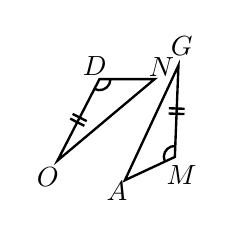
\begin{tikzpicture}

\coordinate (d) at (0,0);  

\coordinate (n) at ($(d) + (0:\lenA)$); 

\coordinate (o) at ($(n) + (-140:2.3*\lenA)$); 

\draw[line width=0.3mm] (d) --  (n) -- (o) -- cycle node[midway] (tick1) {} ; 

%\tikzset{twotick/.pic={\draw[line width=0.3mm] ($(-0.08,0)+(0,0.1*\lenA)$) -- ($(-0.08,0)-(0,0.1*\lenA)$) ($(0.08,0)+(0,0.1*\lenA)$) -- ($(0.08,0)-(0,0.1*\lenA)$) ; }}

\tikzset{twotick/.pic={\draw[line width=0.3mm] ($(-0.02*\lentick,0)+(0,0.06*\lentick)$) -- ($(-0.02*\lentick,0)-(0,0.06*\lentick)$) ($(0.02*\lentick,0)+(0,0.06*\lentick)$) -- ($(0.02*\lentick,0)-(0,0.06*\lentick)$) ; }}  

%\tikzset{twotick/.pic={\draw[line width=0.3mm] ($(-0.02*\lentick)+(0,0.06*\lentick)$) -- ($(-0.02*\lentick,0)-(0,0.06*\lentick)$) ($(0.02*\lentick,0)+(0,0.06*\lentick)$) -- ($(0.02*\lentick,0)-(0,0.06*\lentick)$) ; }}  


\pic[rotate=63] at (tick1) [pic type = twotick]; 

\pic [draw, line width=0.3mm, angle radius=0.2*\lenA] {angle=o--d--n}; 

\node(d-label) at ($(d)+(110:0.25*\lenA)$) {$ D$}; 

\node(n-label) at ($(n)+(60:0.25*\lenA)$) {$ N$}; 

\node(o-label) at ($(o)-(60:0.35*\lenA)$) {$ O$}; 

\coordinate (g) at ($(n) + (30:0.5*\lenA)$); 

\coordinate (a) at ($(g) + (245:2.3*\lenA)$); 

\coordinate (m) at ($(a) + (25:\lenA)$); 

\node(g-label) at ($(g)+(80:0.35*\lenA)$) {$ G$};

\node(m-label) at ($(m)+(-70:0.35*\lenA)$) {$ M$};

\node(a-label) at ($(a)+(235:0.25*\lenA)$) {$ A$}; 

\draw[line width=0.3mm] (g) -- (a)--(m) -- cycle node[midway] (tick2) {} ; 

\pic[rotate=88] at (tick2) [pic type = twotick];  

\pic [draw, line width=0.3mm, angle radius=0.2*\lenA] {angle=g--m--a}; 

\end{tikzpicture} 

\vspace*{3ex} 
%2
\item[2. ] SSS\\
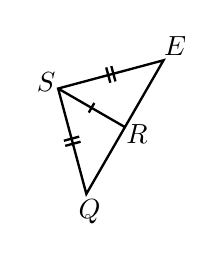
\begin{tikzpicture}

\coordinate (s) at (0,0);  

\coordinate (r) at ($(s) + (-30:1.4*\lenA)$); 

\coordinate (q) at ($(r)!1!90:(s)$); 

\coordinate (e) at ($(r)!1!-90:(s)$); 

\draw[line width=0.3mm] (s)--(q) node[midway] (tick2) {} --(e) -- cycle node[midway] (tick3) {}  (s) --(r) node[midway] (tick1) {} ; 

\node(s-label) at ($(s)+(150:0.25*\lenA)$) {$ S$}; 

\node(q-label) at ($(q)+(280:0.33*\lenA)$) {$ Q$}; 

\node(r-label) at ($(r)+(-30:0.25*\lenA)$) {$ R$}; 

\node(e-label) at ($(e)+(50:0.33*\lenA)$) {$ E$}; 

\tikzset{onetick/.pic={\draw[line width=0.3mm] ($(0,0)+(0,0.1*\lenA)$) -- ($(0,0)-(0,0.1*\lenA)$) ; }}

\pic[rotate=-30] at (tick1) [pic type = onetick]; 

%\tikzset{twotick/.pic={\draw[line width=0.3mm] ($(-0.08,0)+(0,0.1*\lenA)$) -- ($(-0.08,0)-(0,0.1*\lenA)$) ($(0.08,0)+(0,0.1*\lenA)$) -- ($(0.08,0)-(0,0.1*\lenA)$) ; }}

%\tikzset{twotick/.pic={\draw[line width=0.3mm] ($(-0.02*\lenA,0)+(0,0.06*\lenA)$) -- ($(-0.02*\lenA,0)-(0,0.06*\lenA)$) ($(0.02*\lenA,0)+(0,0.06*\lenA)$) -- ($(0.02*\lenA,0)-(0,0.06*\lenA)$) ; }}  

\tikzset{twotick/.pic={\draw[line width=0.3mm] ($(-0.02*\lentick,0)+(0,0.06*\lentick)$) -- ($(-0.02*\lentick,0)-(0,0.06*\lentick)$) ($(0.02*\lentick,0)+(0,0.06*\lentick)$) -- ($(0.02*\lentick,0)-(0,0.06*\lentick)$) ; }}  



\pic[rotate=105] at (tick2) [pic type = twotick];  

\pic[rotate=15] at (tick3) [pic type = twotick];  

\end{tikzpicture} 
 %\\[-1ex]

\end{multicols} 
\end{enumerate} 

\vspace*{-6ex}

\begin{enumerate}[label = \arabic*. ]
\begin{multicols}{3}
%3
\item[3. ] SSS\\
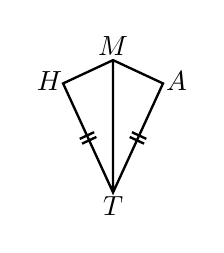
\begin{tikzpicture}

\coordinate (m) at (0,0); 

\coordinate (a) at ($(m) + (-25:\lenA)$); 

\coordinate (h) at ($(m) + (205:\lenA)$); 

\coordinate (t) at ($(m) + (-90:2.4*\lenA)$); 

\node(m-label) at ($(m)+(90:0.25*\lenA)$) {$ M$};

\node(a-label) at ($(a)+(10:0.25*\lenA)$) {$ A$}; 

\node(t-label) at ($(t)+(-90:0.25*\lenA)$) {$ T$};

\node(h-label) at ($(h)+(170:0.25*\lenA)$) {$ H$};

\draw[line width=0.3mm] (m)--(a) -- (t) node[midway] (tick1) {} --(h) node[midway] (tick2) {} -- cycle  (m)--(t); 

%\tikzset{twotick/.pic={\draw[line width=0.3mm] ($(-0.08,0)+(0,0.1*\lenA)$) -- ($(-0.08,0)-(0,0.1*\lenA)$) ($(0.08,0)+(0,0.1*\lenA)$) -- ($(0.08,0)-(0,0.1*\lenA)$) ; }}

%\tikzset{twotick/.pic={\draw[line width=0.3mm] ($(-0.02*\lenA,0)+(0,0.06*\lenA)$) -- ($(-0.02*\lenA,0)-(0,0.06*\lenA)$) ($(0.02*\lenA,0)+(0,0.06*\lenA)$) -- ($(0.02*\lenA,0)-(0,0.06*\lenA)$) ; }}  

\tikzset{twotick/.pic={\draw[line width=0.3mm] ($(-0.02*\lentick,0)+(0,0.06*\lentick)$) -- ($(-0.02*\lentick,0)-(0,0.06*\lentick)$) ($(0.02*\lentick,0)+(0,0.06*\lentick)$) -- ($(0.02*\lentick,0)-(0,0.06*\lentick)$) ; }}  



\pic[rotate=65] at (tick1) [pic type = twotick]; 

\pic[rotate=115] at (tick2) [pic type = twotick]; 

\end{tikzpicture} 


%4
\item[4. ] ASA\\
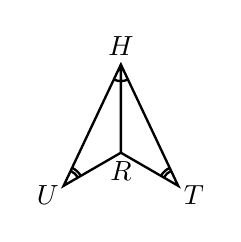
\begin{tikzpicture}

\coordinate (h) at (0,0); 

\coordinate (r) at ($(h) + (-90:1.6*\lenA)$); 

\coordinate (t) at ($(r) + (-30:1.2*\lenA)$); 

\coordinate (u) at ($(r) + (210:1.2*\lenA)$); 

\node(r-label) at ($(r)+(-90:0.33*\lenA)$) {$ R$}; 

\node(t-label) at ($(t)+(-30:0.33*\lenA)$) {$ T$}; 

\node(h-label) at ($(h)+(90:0.33*\lenA)$) {$ H$}; 

\node(u-label) at ($(u)+(210:0.33*\lenA)$) {$ U$}; 

\draw[line width=0.3mm] (h)--(t) --(r) --(u) -- cycle (h) --(r) ; 

\pic [draw, line width=0.3mm, angle radius=0.3*\lenA] {angle=u--h--r}; 

\pic [draw, line width=0.3mm, angle radius=0.3*\lenA] {angle=r--h--t}; 

\pic [draw, line width=0.3mm, angle radius=0.3*\lenA] {angle=r--u--h}; 

\pic [draw, line width=0.3mm, angle radius=0.36*\lenA] {angle=r--u--h}; 

\pic [draw, line width=0.3mm, angle radius=0.3*\lenA] {angle=h--t--r}; 

\pic [draw, line width=0.3mm, angle radius=0.36*\lenA] {angle=h--t--r}; 

\end{tikzpicture} 


%5
\item[5. ] SAS\\
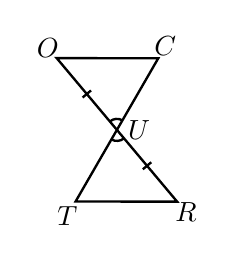
\begin{tikzpicture}

\coordinate (u) at (0,0); 

\coordinate (c) at ($(u) + (60:1.5*\lenA)$); 

\coordinate (t) at ($(u) - (60:1.5*\lenA)$); 

\coordinate (o) at ($(u) + (130:1.7*\lenA)$); 

\coordinate (r) at ($(u) - (130:1.7*\lenA)$); 

\node(u-label) at ($(u)+(0:0.4*\lenA)$) {$ U$};

\node(c-label) at ($(c)+(60:0.25*\lenA)$) {$ C$};

\node(o-label) at ($(o)+(130:0.25*\lenA)$) {$ O$};

\node(t-label) at ($(t)-(60:0.3*\lenA)$) {$ T$};

\node(r-label) at ($(r)-(130:0.25*\lenA)$) {$ R$}; 

\draw[line width=0.3mm] (u)--(o) node[midway] (tick1) {} --(c)--(t)--(r)--cycle node[midway] (tick2) {} ; 

\tikzset{onetick/.pic={\draw[line width=0.3mm] ($(0,0)+(0,0.1*\lenA)$) -- ($(0,0)-(0,0.1*\lenA)$) ; }}

\pic[rotate=-50] at (tick1) [pic type = onetick]; 

\pic[rotate=-50] at (tick2) [pic type = onetick]; 

\pic [draw, line width=0.3mm, angle radius=0.2*\lenA] {angle=c--u--o}; 

\pic [draw, line width=0.3mm, angle radius=0.2*\lenA] {angle=t--u--r}; 

\end{tikzpicture} 



\end{multicols} 

\end{enumerate} 

B. Fill in the blanks then indicate the congruence postulate used. 

\begin{enumerate}[label = \arabic*. ]
\begin{multicols}{3}
%1
\item 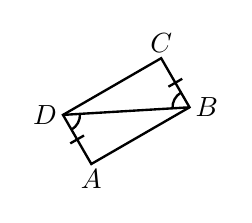
\begin{tikzpicture}

\def\len1{1.2*\lenB}

\draw[line width=0.3mm] 
(0,0) coordinate (a) --++ 
(30:\len1) coordinate (b) --++ 
(120:0.5*\len1) coordinate (c) --++ 
(210:\len1) coordinate (d) -- cycle ;  

\node[anchor=north, inner sep=2pt, rotate=0] (a-label) at (a) {$ A$};

\node[anchor=west, inner sep=2pt, rotate=0] (b-label) at (b) {$ B$}; 

\node[anchor=south, inner sep=2pt, rotate=0] (c-label) at (c) {$ C$};

\node[anchor=east, inner sep=2pt, rotate=0] (d-label) at (d) {$ D$};

\draw[line width=0.3mm] (b) -- (d);  

\coordinate (tick1) at ($(a)!0.5!(d)$) {}; 

\coordinate (tick2) at ($(c)!0.5!(b)$) {};  

\tikzset{onetick/.pic={\draw[line width=0.3mm] ($(0,0)+(0,0.07*\len1)$) -- ($(0,0)-(0,0.07*\len1)$) ; }}

\pic[rotate=-60] at (tick1) [pic type = onetick];  

\pic[rotate=-60] at (tick2) [pic type = onetick];  

\pic [draw, line width=0.3mm, angle radius=0.15*\len1] {angle=c--b--d}; 

\pic [draw, line width=0.3mm, angle radius=0.15*\len1] {angle=a--d--b}; 

\end{tikzpicture} 
%2
\item 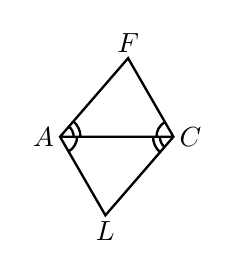
\begin{tikzpicture}

\def\len2{1.2*\lenB}

\draw[line width=0.3mm] (0,0) coordinate (a) -- (-60:0.8*\len2) coordinate (l) -- (0:\len2) coordinate (c)  --++ (120:0.8*\len2) coordinate (f) -- cycle -- (c) ;  

\node[anchor=east, inner sep=2pt, rotate=0] (a-label) at (a) {$ A$};

\node[anchor=north, inner sep=2pt, rotate=0] (l-label) at (l) {$ L$}; 

\node[anchor=west, inner sep=2pt, rotate=0] (c-label) at (c) {$ C$};

\node[anchor=south, inner sep=2pt, rotate=0] (f-label) at (f) {$ F$};

\pic [draw, line width=0.3mm, angle radius=0.15*\len2] {angle=l--a--c}; 

\pic [draw, line width=0.3mm, angle radius=0.18*\len2] {angle=a--c--l}; 

\pic [draw, line width=0.3mm, angle radius=0.12*\len2] {angle=a--c--l}; 

\pic [draw, line width=0.3mm, angle radius=0.15*\len2] {angle=f--c--a}; 

\pic [draw, line width=0.3mm, angle radius=0.12*\len2] {angle=c--a--f}; 

\pic [draw, line width=0.3mm, angle radius=0.18*\len2] {angle=c--a--f}; 

\end{tikzpicture} 
%3
\item 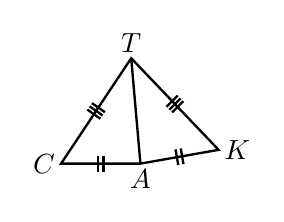
\begin{tikzpicture}

\def\len3{1.4*\lenB}

\draw[line width=0.3mm] (0,0) coordinate (a) -- (10:0.6*\len3) coordinate (k) -- (95:0.8*\len3) coordinate (t) -- (180:0.6*\len3) coordinate (c) -- cycle --  (t);  

\node[anchor=north, inner sep=2pt, rotate=0] (a-label) at (a) {$ A$};

\node[anchor=south, inner sep=2pt, rotate=0] (t-label) at (t) {$ T$}; 

\node[anchor=east, inner sep=2pt, rotate=0] (c-label) at (c) {$ C$};

\node[anchor=west, inner sep=2pt, rotate=0] (k-label) at (k) {$ K$};

\coordinate (tick1) at ($(a)!0.5!(c)$) {};  

\tikzset{twotick/.pic={\draw[line width=0.3mm] ($(-0.02*\lentick,0)+(0,0.06*\lentick)$) -- ($(-0.02*\lentick,0)-(0,0.06*\lentick)$) ($(0.02*\lentick,0)+(0,0.06*\lentick)$) -- ($(0.02*\lentick,0)-(0,0.06*\lentick)$) ; }}  
  

\tikzset{threetick/.pic={\draw[line width=0.3mm] ($(-0.03*\len3,0)+(0,0.06*\len3)$) -- ($(-0.03*\len3,0)-(0,0.06*\len3)$) ($(0,0)+(0,0.06*\len3)$) -- ($(0,0)-(0,0.06*\len3)$)  ($(0.03*\len3,0)+(0,0.06*\len3)$) -- ($(0.03*\len3,0)-(0,0.06*\len3)$) ; }}

\pic[rotate=0] at (tick1) [pic type = twotick];  

\coordinate (tick2) at ($(t)!0.5!(c)$) {};

\coordinate (tick3) at ($(a)!0.5!(k)$) {};  

\coordinate (tick4) at ($(t)!0.5!(k)$) {};

\tikzset{onetick/.pic={\draw[line width=0.3mm] ($(0,0)+(0,0.06*\len3)$) -- ($(0,0)-(0,0.06*\len3)$) ; }}

%\pic[rotate=60] at (tick2) [pic type = onetick];

\pic[rotate=55] at (tick2) [pic type = threetick];

\pic[rotate=10] at (tick3) [pic type = twotick];

\pic[rotate=-45] at (tick4) [pic type = threetick];  

\end{tikzpicture} 

\end{multicols} 
\end{enumerate}  
 


%\def\figdir{/storage/emulated/0/Documents/documents/latex/1920/Grade-8/3rd/triangle-congruence-postulates/f}


\begin{enumerate}[label = \arabic*. ]
\begin{multicols}{2}
%4
\item[4. ] 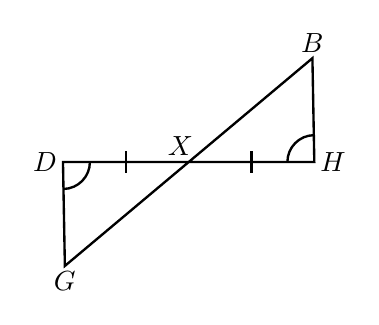
\begin{tikzpicture}

\def\len4{1.9*\lenB}

\draw[line width=0.3mm] (0,0) coordinate (x) -- (40:0.9*\len4) coordinate (b) -- (0:0.7*\len4) coordinate (h) -- (180:0.7*\len4) coordinate (d) -- (220:0.9*\len4) coordinate (g) -- cycle; 

\node[xshift=-3pt, anchor=south, inner sep=2pt, rotate=0] (x-label) at (x) {$ X$};

\node[anchor=south, inner sep=2pt, rotate=0] (b-label) at (b) {$ B$}; 

\node[anchor=west, inner sep=2pt, rotate=0] (h-label) at (h) {$ H$};

\node[anchor=east, inner sep=2pt, rotate=0] (d-label) at (d) {$ D$};

\node[anchor=north, inner sep=2pt, rotate=0] (g-label) at (g) {$ G$};

\coordinate (tick1) at ($(x)!0.5!(h)$) {}; 

\coordinate (tick2) at ($(x)!0.5!(d)$) {};  

\tikzset{onetick/.pic={\draw[line width=0.3mm] ($(0,0)+(0,0.06*\len4)$) -- ($(0,0)-(0,0.06*\len4)$) ; }}

\pic[rotate=0] at (tick1) [pic type = onetick];

\pic[rotate=0] at (tick2) [pic type = onetick];   

\pic [draw, line width=0.3mm, angle radius=0.15*\len4] {angle=b--h--x}; 

\pic [draw, line width=0.3mm, angle radius=0.15*\len4] {angle=g--d--x}; 

\end{tikzpicture} 
%5 
\item[5. ] 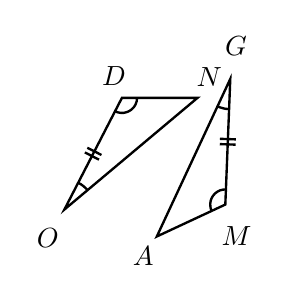
\begin{tikzpicture}

\def\len5{0.8*\lenB}

\coordinate (d) at (0,0);  

\coordinate (n) at ($(d) + (0:\len5)$); 

\coordinate (o) at ($(n) + (-140:2.3*\len5)$); 

\draw[line width=0.3mm] (d) --  (n) -- (o) -- cycle node[midway] (tick1) {} ; 

%\tikzset{twotick/.pic={\draw[line width=0.3mm] ($(-0.03*\len5,0)+(0,0.1*\len5)$) -- ($(-0.03*\len5,0)-(0,0.1*\len5)$) ($(0.03*\len5,0)+(0,0.1*\len5)$) -- ($(0.03*\len5,0)-(0,0.1*\len5)$) ; }}
\tikzset{twotick/.pic={\draw[line width=0.3mm] ($(-0.02*\lentick,0)+(0,0.06*\lentick)$) -- ($(-0.02*\lentick,0)-(0,0.06*\lentick)$) ($(0.02*\lentick,0)+(0,0.06*\lentick)$) -- ($(0.02*\lentick,0)-(0,0.06*\lentick)$) ; }}  


%\tikzset{twotick/.pic={\draw[line width=0.3mm] ($(-0.02*\len5,0)+(0,0.06*\len5)$) -- ($(-0.02*\len5,0)-(0,0.06*\len5)$) ($(0.02*\len5,0)+(0,0.06*\len5)$) -- ($(0.02*\len5,0)-(0,0.06*\len5)$) ; }}  

\pic[rotate=63] at (tick1) [pic type = twotick]; 

\pic [draw, line width=0.3mm, angle radius=0.2*\len5] {angle=o--d--n}; 

\node(d-label) at ($(d)+(110:0.25*\lenB)$) {$ D$}; 

\node(n-label) at ($(n)+(60:0.25*\lenB)$) {$ N$}; 

\node(o-label) at ($(o)-(60:0.35*\lenB)$) {$ O$}; 

\coordinate (g) at ($(n) + (30:0.5*\len5)$); 

\coordinate (a) at ($(g) + (245:2.3*\len5)$); 

\coordinate (m) at ($(a) + (25:\len5)$); 

\node(g-label) at ($(g)+(80:0.35*\lenB)$) {$ G$};

\node(m-label) at ($(m)+(-70:0.35*\lenB)$) {$ M$};

\node(a-label) at ($(a)+(235:0.25*\lenB)$) {$ A$}; 

\draw[line width=0.3mm] (g) -- (a)--(m) -- cycle node[midway] (tick2) {} ; 

\pic[rotate=88] at (tick2) [pic type = twotick];  

\pic [draw, line width=0.3mm, angle radius=0.2*\len5] {angle=g--m--a}; 

\pic [draw, line width=0.3mm, angle radius=0.4*\len5] {angle=a--g--m}; 

\pic [draw, line width=0.3mm, angle radius=0.4*\len5] {angle=n--o--d}; 

\end{tikzpicture} 

\end{multicols} 
\end{enumerate}  
 


\begin{enumerate}[label = \arabic*. ]
\begin{multicols}{3}

%1
\item $\overline{CB} \cong$ \blank \\
$\overline{BD} \cong$ \blank \\
$\angle{CBD} \cong$ \blank \\
$\triangle{CBD} \cong$ \blank \\
Postulate: \blank
%2
\item $\overline{AC} \cong$ \blank \\
$\angle{FCA} \cong$ \blank \\
$\angle{FAC} \cong$ \blank \\
$\triangle{FCA} \cong$ \blank \\
Postulate: \blank
%3
\item $\overline{AT} \cong$ \blank \\
$\overline{AC} \cong$ \blank \\
$\overline{CT} \cong$ \blank \\
$\triangle{ACT} \cong$ \blank \\
Postulate: \blank
%4
\item $\overline{DX} \cong$ \blank \\
$\angle{DXG} \cong$ \blank \\
$\angle{D} \cong$ \blank \\
$\triangle{DXG} \cong$ \blank \\
Postulate: \blank
%5
\item $\overline{DO} \cong$ \blank \\
$\angle{O} \cong$ \blank \\
$\angle{D} \cong$ \blank \\
$\triangle{DON} \cong$ \blank \\
Postulate: \blank

\end{multicols} 
\end{enumerate}   
%}}

%\vspace*{1ex}
%\def\figdir{/storage/emulated/0/Documents/documents/latex/1920/Grade-8/3rd/triangle-congruence-postulates/f}


%\textbf{Practice Exercises}
\textbf{Problem Set}

\vspce
A. Fill in the blanks then indicate the congruence postulate used. 

%\begin{center}
%\vspace*{2ex}
%\scalebox{1}{
%\noindent\begin{minipage}{\textwidth}
{\begin{enumerate}[label = \arabic*. ]
\begin{multicols}{3}
%1
\item 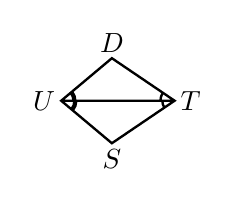
\begin{tikzpicture}

\def\len1{\lenB}

\draw[line width=0.3mm] (0,0) coordinate (u)  -- (40:0.7*\len1) coordinate (d) -- (0:1.2*\len1) coordinate (t) -- (-40:0.7*\len1) coordinate (s) -- cycle -- (t) ;  

\node[anchor=east, inner sep=2pt, rotate=0] (u-label) at (u) {$ U$}; 

\node[anchor=south, inner sep=2pt, rotate=0] (d-label) at (d) {$ D$}; 

\node[anchor=west, inner sep=2pt, rotate=0] (t-label) at (t) {$ T$}; 

\node[anchor=north, inner sep=2pt, rotate=0] (s-label) at (s) {$ S$}; 

\pic [draw, line width=0.3mm, angle radius=0.15*\len1] {angle=d--t--u}; 

\pic [draw, line width=0.3mm, angle radius=0.13*\len1] {angle=u--t--s}; 

\pic [draw, line width=0.3mm, angle radius=0.14*\len1] {angle=s--u--t}; 

\pic [draw, line width=0.3mm, angle radius=0.16*\len1] {angle=s--u--t}; 

\pic [draw, line width=0.3mm, angle radius=0.13*\len1] {angle=t--u--d}; 

\pic [draw, line width=0.3mm, angle radius=0.15*\len1] {angle=t--u--d}; 

\end{tikzpicture} 
%2
\item 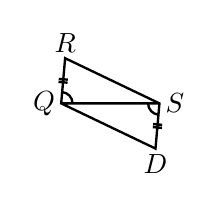
\begin{tikzpicture}

\def\len2{0.8*\lenB}

\draw[line width=0.3mm] (0,0) coordinate (q)  -- (85:0.6*\len2) coordinate (r) -- (0:1.3*\len2) coordinate (s) --++ (-95:0.6*\len2) coordinate (d) -- cycle --(s) ;  

\node[anchor=east, inner sep=2pt, rotate=0] (q-label) at (q) {$ Q$}; 

\node[anchor=south, inner sep=2pt, rotate=0] (r-label) at (r) {$ R$}; 

\node[anchor=west, inner sep=2pt, rotate=0] (s-label) at (s) {$ S$}; 

\node[anchor=north, inner sep=2pt, rotate=0] (d-label) at (d) {$ D$}; 

\coordinate (tick1) at ($(q)!0.5!(r)$) {};

\coordinate (tick2) at ($(s)!0.5!(d)$) {};  

\tikzset{twotick/.pic={\draw[line width=0.3mm] ($(-0.02*\len2, 0)+(0, 0.06*\len2)$) -- ($(-0.02*\len2, 0)-(0, 0.06*\len2)$) ($(0.02*\len2, 0)+(0, 0.06*\len2)$) -- ($(0.02*\len2, 0)-(0, 0.06*\len2)$) ; }}

\pic[rotate=85] at (tick1) [pic type = twotick];  

\pic[rotate=85] at (tick2) [pic type = twotick];   

\pic [draw, line width=0.3mm, angle radius=0.15*\len2] {angle=s--q--r}; 

\pic [draw, line width=0.3mm, angle radius=0.15*\len2] {angle=q--s--d}; 

\end{tikzpicture} 
%3
\item 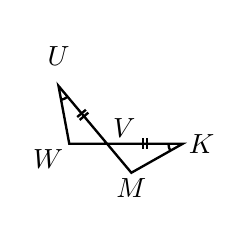
\begin{tikzpicture}%[remember picture, overlay] 

\def\len3{\lenB}

\draw[line width=0.3mm] (0,0) coordinate (v)  -- (130:0.8*\len3) coordinate (u) -- (180:0.4*\len3) coordinate (w) -- (0:0.8*\len3) coordinate (k) -- (-50:0.4*\len3) coordinate (m) -- cycle;  

\node[anchor=south west, inner sep=2pt, rotate=0] (v-label) at (v) {$ V$}; 

\node[anchor=south, inner sep=7pt, rotate=0] (u-label) at (u) {$ U$}; 

\node[anchor=north east, inner sep=2pt, rotate=0] (w-label) at (w) {$ W$}; 

\node[anchor=west, inner sep=2pt, rotate=0] (k-label) at (k) {$ K$}; 

\node[anchor=north, inner sep=2pt, rotate=0] (m-label) at (m) {$ M$}; 

\coordinate (tick1) at ($(u)!0.5!(v)$) {}; 

\coordinate (tick2) at ($(k)!0.5!(v)$) {};  

\tikzset{twotick/.pic={\draw[line width=0.3mm] ($(-0.02*\len3, 0)+(0, 0.06*\len3)$) -- ($(-0.02*\len3, 0)-(0, 0.06*\len3)$) ($(0.02*\len3, 0)+(0, 0.06*\len3)$) -- ($(0.02*\len3, 0)-(0, 0.06*\len3)$) ; }}

\pic[rotate=130] at (tick1) [pic type = twotick];

\pic[rotate=0] at (tick2) [pic type = twotick];   

\pic [draw, line width=0.3mm, angle radius=0.15*\len3] {angle=w--u--v}; 

\pic [draw, line width=0.3mm, angle radius=0.15*\len3] {angle=v--k--m}; 

\end{tikzpicture} 
%4
\item 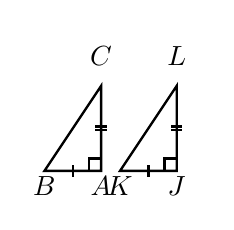
\begin{tikzpicture}

\def\len4{\lenB}

\draw[line width=0.3mm] (0,0) coordinate (a)  -- (180:0.6*\len4) coordinate (b) -- (90:0.9*\len4) coordinate (c) -- cycle;  

\node[anchor=north, inner sep=2pt, rotate=0] (a-label) at (a) {$ A$}; 

\node[anchor=north, inner sep=2pt, rotate=0] (b-label) at (b) {$ B$}; 

\node[anchor=south, inner sep=7pt, rotate=0] (c-label) at (c) {$ C$}; 

\draw[line width=0.3mm, xshift=0.8*\len4] (0,0) coordinate (j)  -- (180:0.6*\len4) coordinate (k) -- (90:0.9*\len4) coordinate (l) -- cycle;

\node[anchor=north, inner sep=2pt, rotate=0] (j-label) at (j) {$ J$}; 

\node[anchor=north, inner sep=2pt, rotate=0] (k-label) at (k) {$ K$}; 

\node[anchor=south, inner sep=7pt, rotate=0] (l-label) at (l) {$ L$}; 

\coordinate (tick1) at ($(a)!0.5!(b)$) {}; 

\coordinate (tick2) at ($(j)!0.5!(k)$) {};  

\tikzset{onetick/.pic={\draw[line width=0.3mm] ($(0,0)+(0, 0.06*\len4)$) -- ($(0,0)-(0, 0.06*\len4)$) ; }}

\pic[rotate=0] at (tick1) [pic type = onetick]; 

\pic[rotate=0] at (tick2) [pic type = onetick];   

\coordinate (tick3) at ($(a)!0.5!(c)$) {};  

\coordinate (tick4) at ($(l)!0.5!(j)$) {};  

\tikzset{twotick/.pic={\draw[line width=0.3mm] ($(-0.02*\len4, 0)+(0, 0.06*\len4)$) -- ($(-0.02*\len4, 0)-(0, 0.06*\len4)$) ($(0.02*\len4, 0)+(0, 0.06*\len4)$) -- ($(0.02*\len4, 0)-(0, 0.06*\len4)$) ; }}

\pic[rotate=90] at (tick3) [pic type = twotick];

\pic[rotate=90] at (tick4) [pic type = twotick];  

\begin{scope} [rotate=90]
\draw[line width=0.3mm] (a) rectangle ++(0.13*\len4,0.13*\len4) node[transform shape]{};
\end{scope} 

\begin{scope} [rotate=90]
\draw[line width=0.3mm] (j) rectangle ++(0.13*\len4,0.13*\len4) node[transform shape]{};
\end{scope} 

\end{tikzpicture} 
%5
\item 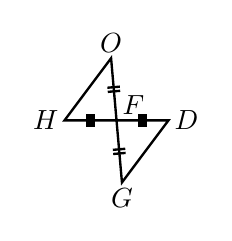
\begin{tikzpicture}

\def\len5{1.1*\lenB}

\draw[line width=0.3mm] (0,0) coordinate (f)  -- (95:0.6*\len5) coordinate (o) -- (180:0.5*\len5) coordinate (h)  -- (0:0.5*\len5) coordinate (d) -- (-85:0.6*\len5) coordinate (g) -- cycle;  

\node[anchor=south west, inner sep=2pt, rotate=0] (f-label) at (f) {$ F$};

\node[anchor=south, inner sep=2pt, rotate=0] (o-label) at (o) {$ O$};

\node[anchor=east, inner sep=2pt, rotate=0] (h-label) at (h) {$ H$};

\node[anchor=west, inner sep=2pt, rotate=0] (d-label) at (d) {$ D$};

\node[anchor=north, inner sep=2pt, rotate=0] (g-label) at (g) {$ G$};

\coordinate (tick1) at ($(o)!0.5!(f)$) {};  

\coordinate (tick2) at ($(f)!0.5!(g)$) {};  

\tikzset{twotick/.pic={\draw[line width=0.3mm] ($(-0.02*\len5, 0)+(0, 0.06*\len5)$) -- ($(-0.02*\len5, 0)-(0, 0.06*\len5)$) ($(0.02*\len5, 0)+(0, 0.06*\len5)$) -- ($(0.02*\len5, 0)-(0, 0.06*\len5)$) ; }}

\pic[rotate=95] at (tick1) [pic type = twotick]; 

\pic[rotate=95] at (tick2) [pic type = twotick];   

\coordinate (tick3) at ($(h)!0.5!(f)$) {};  

\coordinate (tick4) at ($(f)!0.5!(d)$) {};  

\tikzset{threetick/.pic={\draw[line width=0.3mm] ($(-0.03*\len5, 0)+(0, 0.06*\len5)$) -- ($(-0.03*\len5, 0)-(0, 0.06*\len5)$) ($(0,0)+(0, 0.06*\len5)$) -- ($(0,0)-(0, 0.06*\len5)$)  ($(0.03*\len5, 0)+(0, 0.06*\len5)$) -- ($(0.03*\len5, 0)-(0, 0.06*\len5)$) ; }}

\pic[rotate=0] at (tick3) [pic type = threetick]; 

\pic[rotate=0] at (tick4) [pic type = threetick];   

\end{tikzpicture} 
%6
\item 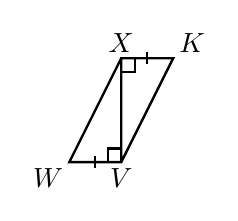
\begin{tikzpicture}

\def\len6{1.1*\lenB}

\draw[line width=0.3mm] (0,0) coordinate (v)  -- (180:0.5*\len6) coordinate (w) -- (90:\len6) coordinate (x) --++ (0:0.5*\len6) coordinate (k) -- cycle -- (x) ; 

\node[anchor=north, inner sep=2pt, rotate=0] (v-label) at (v) {$ V$};

\node[anchor=north east, inner sep=2pt, rotate=0] (w-label) at (w) {$ W$};

\node[anchor=south, inner sep=2pt, rotate=0] (x-label) at (x) {$ X$};

\node[anchor=south west, inner sep=2pt, rotate=0] (k-label) at (k) {$ K$};

\begin{scope} [rotate=90]
\draw[line width=0.3mm] (v) rectangle ++(0.13*\len6,0.13*\len6) node[transform shape]{};
\end{scope} 

\begin{scope} [rotate=-90]
\draw[line width=0.3mm] (x) rectangle ++(0.13*\len6,0.13*\len6) node[transform shape]{};
\end{scope} 

\coordinate (tick1) at ($(w)!0.5!(v)$) {};  

\coordinate (tick2) at ($(x)!0.5!(k)$) {};  

\tikzset{onetick/.pic={\draw[line width=0.3mm] ($(0,0)+(0, 0.06*\len6)$) -- ($(0,0)-(0, 0.06*\len6)$) ; }}

\pic[rotate=0] at (tick1) [pic type = onetick];

\pic[rotate=0] at (tick2) [pic type = onetick];   

\end{tikzpicture} 
%7
%\item 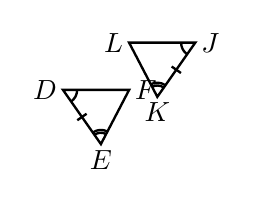
\begin{tikzpicture}

\def\len7{\lenB}

\draw[line width=0.3mm] (0,0) coordinate (d)  -- (-55:0.7*\len7) coordinate (e) -- (0:0.7*\len7) coordinate (f) -- cycle; 

\node[anchor=east, inner sep=2pt, rotate=0] (d-label) at (d) {$ D$};

\node[anchor=north, inner sep=2pt, rotate=0] (e-label) at (e) {$ E$};

\node[anchor=west, inner sep=2pt, rotate=0] (f-label) at (f) {$ F$};

\draw[line width=0.3mm, xshift=0.7*\len7, yshift=0.5*\len7, remember picture, overlay]  (0,0) coordinate (l) -- (0:0.7*\len7) coordinate (j) --++ (235:0.7*\len7) coordinate (k) -- cycle; 

\node[anchor=west, inner sep=2pt, rotate=0] (j-label) at (j) {$ J$};

\node[anchor=north, inner sep=2pt, rotate=0] (k-label) at (k) {$ K$};

\node[anchor=east, inner sep=2pt, rotate=0] (l-label) at (l) {$ L$};

\pic [draw, line width=0.3mm, angle radius=0.15*\len7] {angle=e--d--f};

\pic [draw, line width=0.3mm, angle radius=0.15*\len7] {angle=l--j--k};

\pic [draw, line width=0.3mm, angle radius=0.15*\len7] {angle=f--e--d};

\pic [draw, line width=0.3mm, angle radius=0.12*\len7] {angle=f--e--d};

\pic [draw, line width=0.3mm, angle radius=0.15*\len7] {angle=j--k--l};

\pic [draw, line width=0.3mm, angle radius=0.12*\len7] {angle=j--k--l};

\coordinate (tick1) at ($(d)!0.5!(e)$) {};  

\coordinate (tick2) at ($(j)!0.5!(k)$) {};  

\tikzset{onetick/.pic={\draw[line width=0.3mm] ($(0,0)+(0, 0.06*\len7)$) -- ($(0,0)-(0, 0.06*\len7)$) ; }}

\pic[rotate=-55] at (tick1) [pic type = onetick]; 

\pic[rotate=55] at (tick2) [pic type = onetick];   

\end{tikzpicture} 
%8
%\item 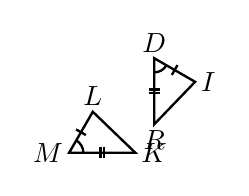
\begin{tikzpicture}

\def\len8{\lenB}

\draw[line width=0.3mm, remember picture, overlay] (0,0) coordinate (m)  -- (60:0.5*\len8) coordinate (l) -- (0:0.7*\len8) coordinate (k) -- cycle; 

\node[anchor=east, inner sep=2pt, rotate=0] (m-label) at (m) {$ M$};

\node[anchor=south, inner sep=2pt, rotate=0] (l-label) at (l) {$ L$};

\node[anchor=west, inner sep=2pt, rotate=0] (k-label) at (k) {$ K$};

\draw[line width=0.3mm, rotate=-90, xshift=-1*\len8,
yshift=0.9*\len8
] (0,0) coordinate (d)  -- (60:0.5*\len8) coordinate (i) -- (0:0.7*\len8) coordinate (r) -- cycle; 

\node[anchor=south, inner sep=2pt, rotate=0] (d-label) at (d) {$ D$};

\node[anchor=west, inner sep=2pt, rotate=0] (i-label) at (i) {$ I$};

\node[anchor=north, inner sep=2pt, rotate=0] (r-label) at (r) {$ R$};

\pic [draw, line width=0.3mm, angle radius=0.15*\len8] {angle=k--m--l}; 

\pic [draw, line width=0.3mm, angle radius=0.15*\len8] {angle=r--d--i}; 

\coordinate (tick1) at ($(l)!0.5!(m)$) {};  

\coordinate (tick2) at ($(d)!0.5!(i)$) {};  

\tikzset{onetick/.pic={\draw[line width=0.3mm] ($(0,0)+(0, 0.06*\len8)$) -- ($(0,0)-(0, 0.06*\len8)$) ; }}

\pic[rotate=60] at (tick1) [pic type = onetick];

\pic[rotate=-30] at (tick2) [pic type = onetick]; 

\coordinate (tick3) at ($(k)!0.5!(m)$) {};  

\coordinate (tick4) at ($(d)!0.5!(r)$) {};  

\tikzset{twotick/.pic={\draw[line width=0.3mm] ($(-0.02*\len8, 0)+(0, 0.06*\len8)$) -- ($(-0.02*\len8, 0)-(0, 0.06*\len8)$) ($(0.02*\len8, 0)+(0, 0.06*\len8)$) -- ($(0.02*\len8, 0)-(0, 0.06*\len8)$) ; }}

\pic[rotate=0] at (tick3) [pic type = twotick];

\pic[rotate=90] at (tick4) [pic type = twotick];    

\end{tikzpicture} 

\end{multicols} 
\end{enumerate}}
%\end{minipage}}
%\end{center}  

    
\begin{enumerate}[label = \arabic*. ]
\begin{multicols}{3}

%1
\item $\overline{TU} \cong$ \blank \\
$\angle{DUT} \cong$ \blank \\
$\angle{DTU} \cong$ \blank \\
$\triangle{DUT} \cong$ \blank \\
Postulate: \blank
%2
\item $\overline{QS} \cong$ \blank \\
$\overline{QR} \cong$ \blank \\
$\angle{RQS} \cong$ \blank \\
$\triangle{RQS} \cong$ \blank \\
Postulate: \blank
%3
\item $\overline{UV} \cong$ \blank \\
$\angle{U} \cong$ \blank \\
$\angle{UVW} \cong$ \blank \\
$\triangle{UVW} \cong$ \blank \\
Postulate: \blank
%4
\item $\overline{AB} \cong$ \blank \\
$\overline{AC} \cong$ \blank \\
$\angle{A} \cong$ \blank \\
$\triangle{ABC} \cong$ \blank \\
Postulate: \blank
%5
\item $\overline{FO} \cong$ \blank \\
$\overline{HF} \cong$ \blank \\
$\angle{HFO} \cong$ \blank \\
$\triangle{HFO} \cong$ \blank \\
Postulate: \blank
%6
\item $\overline{KX} \cong$ \blank \\
$\overline{XV} \cong$ \blank \\
$\angle{KXV} \cong$ \blank \\
$\triangle{KXV} \cong$ \blank \\
Postulate: \blank

\end{multicols} 
\end{enumerate}   
%}}



\end{frame}

% frame 2
\vertadjust
\begin{frame} 
%\begin{center}
\textbf{Triangle Congruence Postulates 
}
\end{center}

\vspce

Included angle: the angle between two sides of a triangle 

\vspce 

Included side: the side common to  two angles  of a triangle 


\vspce 

SSS (Side-Side-Side) Congruence Postulate: If the three sides of one triangle are congruent to the corresponding sides of another triangle, then the two triangles are congruent.

\vspce 

SAS (Side-Angle-Side) Congruence Postulate: 

If the two sides and an included angle of one triangle are congruent to the corresponding  two sides and included angle of another triangle, then the two triangles are congruent.

\vspce 

ASA (Angle-Side-Angle) Congruence Postulate: If two angles and the included side of one triangle are congruent to the corresponding two angles and included side of another triangle, then the two triangles are congruent. 

\vspce 

HL (Hypotenuse-Leg) Congruence Postulate: If the hypotenuse and a leg of one right triangle are congruent to the corresponding hypotenuse and side of another right triangle, then the two right triangles are congruent.



% \\
%\def\figdir{/storage/emulated/0/Documents/documents/latex/1920/Grade-8/3rd/triangle-congruence-postulates/f}

\textbf{Practice Exercises}
%\textbf{Problem Set}

\vspce

%\begin{enumerate}[label = \Alph*. ]
%A
%\item \hspce 
A. The figures are marked with their congruent parts. Determine the other congruent parts to satisfy the condition written for each figure. 

%\begin{multicols}{2}

\begin{enumerate}[label = \arabic*. ]

\begin{multicols}{2}

%1
\item SAS \\
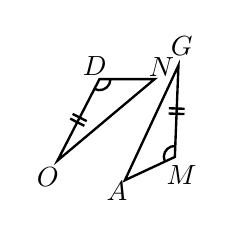
\begin{tikzpicture}

\coordinate (d) at (0,0);  

\coordinate (n) at ($(d) + (0:\lenA)$); 

\coordinate (o) at ($(n) + (-140:2.3*\lenA)$); 

\draw[line width=0.3mm] (d) --  (n) -- (o) -- cycle node[midway] (tick1) {} ; 

%\tikzset{twotick/.pic={\draw[line width=0.3mm] ($(-0.08,0)+(0,0.1*\lenA)$) -- ($(-0.08,0)-(0,0.1*\lenA)$) ($(0.08,0)+(0,0.1*\lenA)$) -- ($(0.08,0)-(0,0.1*\lenA)$) ; }}

\tikzset{twotick/.pic={\draw[line width=0.3mm] ($(-0.02*\lentick,0)+(0,0.06*\lentick)$) -- ($(-0.02*\lentick,0)-(0,0.06*\lentick)$) ($(0.02*\lentick,0)+(0,0.06*\lentick)$) -- ($(0.02*\lentick,0)-(0,0.06*\lentick)$) ; }}  

%\tikzset{twotick/.pic={\draw[line width=0.3mm] ($(-0.02*\lentick)+(0,0.06*\lentick)$) -- ($(-0.02*\lentick,0)-(0,0.06*\lentick)$) ($(0.02*\lentick,0)+(0,0.06*\lentick)$) -- ($(0.02*\lentick,0)-(0,0.06*\lentick)$) ; }}  


\pic[rotate=63] at (tick1) [pic type = twotick]; 

\pic [draw, line width=0.3mm, angle radius=0.2*\lenA] {angle=o--d--n}; 

\node(d-label) at ($(d)+(110:0.25*\lenA)$) {$ D$}; 

\node(n-label) at ($(n)+(60:0.25*\lenA)$) {$ N$}; 

\node(o-label) at ($(o)-(60:0.35*\lenA)$) {$ O$}; 

\coordinate (g) at ($(n) + (30:0.5*\lenA)$); 

\coordinate (a) at ($(g) + (245:2.3*\lenA)$); 

\coordinate (m) at ($(a) + (25:\lenA)$); 

\node(g-label) at ($(g)+(80:0.35*\lenA)$) {$ G$};

\node(m-label) at ($(m)+(-70:0.35*\lenA)$) {$ M$};

\node(a-label) at ($(a)+(235:0.25*\lenA)$) {$ A$}; 

\draw[line width=0.3mm] (g) -- (a)--(m) -- cycle node[midway] (tick2) {} ; 

\pic[rotate=88] at (tick2) [pic type = twotick];  

\pic [draw, line width=0.3mm, angle radius=0.2*\lenA] {angle=g--m--a}; 

\end{tikzpicture} 

\vspace*{3ex} 
%2
\item[2. ] SSS\\
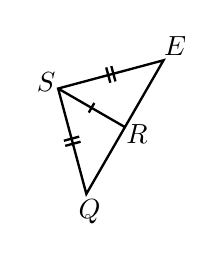
\begin{tikzpicture}

\coordinate (s) at (0,0);  

\coordinate (r) at ($(s) + (-30:1.4*\lenA)$); 

\coordinate (q) at ($(r)!1!90:(s)$); 

\coordinate (e) at ($(r)!1!-90:(s)$); 

\draw[line width=0.3mm] (s)--(q) node[midway] (tick2) {} --(e) -- cycle node[midway] (tick3) {}  (s) --(r) node[midway] (tick1) {} ; 

\node(s-label) at ($(s)+(150:0.25*\lenA)$) {$ S$}; 

\node(q-label) at ($(q)+(280:0.33*\lenA)$) {$ Q$}; 

\node(r-label) at ($(r)+(-30:0.25*\lenA)$) {$ R$}; 

\node(e-label) at ($(e)+(50:0.33*\lenA)$) {$ E$}; 

\tikzset{onetick/.pic={\draw[line width=0.3mm] ($(0,0)+(0,0.1*\lenA)$) -- ($(0,0)-(0,0.1*\lenA)$) ; }}

\pic[rotate=-30] at (tick1) [pic type = onetick]; 

%\tikzset{twotick/.pic={\draw[line width=0.3mm] ($(-0.08,0)+(0,0.1*\lenA)$) -- ($(-0.08,0)-(0,0.1*\lenA)$) ($(0.08,0)+(0,0.1*\lenA)$) -- ($(0.08,0)-(0,0.1*\lenA)$) ; }}

%\tikzset{twotick/.pic={\draw[line width=0.3mm] ($(-0.02*\lenA,0)+(0,0.06*\lenA)$) -- ($(-0.02*\lenA,0)-(0,0.06*\lenA)$) ($(0.02*\lenA,0)+(0,0.06*\lenA)$) -- ($(0.02*\lenA,0)-(0,0.06*\lenA)$) ; }}  

\tikzset{twotick/.pic={\draw[line width=0.3mm] ($(-0.02*\lentick,0)+(0,0.06*\lentick)$) -- ($(-0.02*\lentick,0)-(0,0.06*\lentick)$) ($(0.02*\lentick,0)+(0,0.06*\lentick)$) -- ($(0.02*\lentick,0)-(0,0.06*\lentick)$) ; }}  



\pic[rotate=105] at (tick2) [pic type = twotick];  

\pic[rotate=15] at (tick3) [pic type = twotick];  

\end{tikzpicture} 
 %\\[-1ex]

\end{multicols} 
\end{enumerate} 

\vspace*{-6ex}

\begin{enumerate}[label = \arabic*. ]
\begin{multicols}{3}
%3
\item[3. ] SSS\\
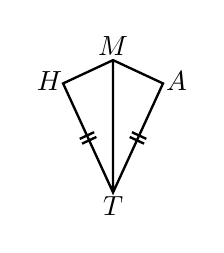
\begin{tikzpicture}

\coordinate (m) at (0,0); 

\coordinate (a) at ($(m) + (-25:\lenA)$); 

\coordinate (h) at ($(m) + (205:\lenA)$); 

\coordinate (t) at ($(m) + (-90:2.4*\lenA)$); 

\node(m-label) at ($(m)+(90:0.25*\lenA)$) {$ M$};

\node(a-label) at ($(a)+(10:0.25*\lenA)$) {$ A$}; 

\node(t-label) at ($(t)+(-90:0.25*\lenA)$) {$ T$};

\node(h-label) at ($(h)+(170:0.25*\lenA)$) {$ H$};

\draw[line width=0.3mm] (m)--(a) -- (t) node[midway] (tick1) {} --(h) node[midway] (tick2) {} -- cycle  (m)--(t); 

%\tikzset{twotick/.pic={\draw[line width=0.3mm] ($(-0.08,0)+(0,0.1*\lenA)$) -- ($(-0.08,0)-(0,0.1*\lenA)$) ($(0.08,0)+(0,0.1*\lenA)$) -- ($(0.08,0)-(0,0.1*\lenA)$) ; }}

%\tikzset{twotick/.pic={\draw[line width=0.3mm] ($(-0.02*\lenA,0)+(0,0.06*\lenA)$) -- ($(-0.02*\lenA,0)-(0,0.06*\lenA)$) ($(0.02*\lenA,0)+(0,0.06*\lenA)$) -- ($(0.02*\lenA,0)-(0,0.06*\lenA)$) ; }}  

\tikzset{twotick/.pic={\draw[line width=0.3mm] ($(-0.02*\lentick,0)+(0,0.06*\lentick)$) -- ($(-0.02*\lentick,0)-(0,0.06*\lentick)$) ($(0.02*\lentick,0)+(0,0.06*\lentick)$) -- ($(0.02*\lentick,0)-(0,0.06*\lentick)$) ; }}  



\pic[rotate=65] at (tick1) [pic type = twotick]; 

\pic[rotate=115] at (tick2) [pic type = twotick]; 

\end{tikzpicture} 


%4
\item[4. ] ASA\\
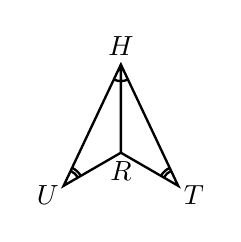
\begin{tikzpicture}

\coordinate (h) at (0,0); 

\coordinate (r) at ($(h) + (-90:1.6*\lenA)$); 

\coordinate (t) at ($(r) + (-30:1.2*\lenA)$); 

\coordinate (u) at ($(r) + (210:1.2*\lenA)$); 

\node(r-label) at ($(r)+(-90:0.33*\lenA)$) {$ R$}; 

\node(t-label) at ($(t)+(-30:0.33*\lenA)$) {$ T$}; 

\node(h-label) at ($(h)+(90:0.33*\lenA)$) {$ H$}; 

\node(u-label) at ($(u)+(210:0.33*\lenA)$) {$ U$}; 

\draw[line width=0.3mm] (h)--(t) --(r) --(u) -- cycle (h) --(r) ; 

\pic [draw, line width=0.3mm, angle radius=0.3*\lenA] {angle=u--h--r}; 

\pic [draw, line width=0.3mm, angle radius=0.3*\lenA] {angle=r--h--t}; 

\pic [draw, line width=0.3mm, angle radius=0.3*\lenA] {angle=r--u--h}; 

\pic [draw, line width=0.3mm, angle radius=0.36*\lenA] {angle=r--u--h}; 

\pic [draw, line width=0.3mm, angle radius=0.3*\lenA] {angle=h--t--r}; 

\pic [draw, line width=0.3mm, angle radius=0.36*\lenA] {angle=h--t--r}; 

\end{tikzpicture} 


%5
\item[5. ] SAS\\
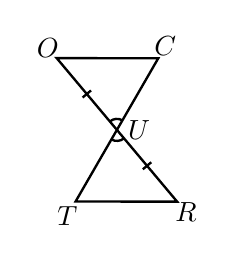
\begin{tikzpicture}

\coordinate (u) at (0,0); 

\coordinate (c) at ($(u) + (60:1.5*\lenA)$); 

\coordinate (t) at ($(u) - (60:1.5*\lenA)$); 

\coordinate (o) at ($(u) + (130:1.7*\lenA)$); 

\coordinate (r) at ($(u) - (130:1.7*\lenA)$); 

\node(u-label) at ($(u)+(0:0.4*\lenA)$) {$ U$};

\node(c-label) at ($(c)+(60:0.25*\lenA)$) {$ C$};

\node(o-label) at ($(o)+(130:0.25*\lenA)$) {$ O$};

\node(t-label) at ($(t)-(60:0.3*\lenA)$) {$ T$};

\node(r-label) at ($(r)-(130:0.25*\lenA)$) {$ R$}; 

\draw[line width=0.3mm] (u)--(o) node[midway] (tick1) {} --(c)--(t)--(r)--cycle node[midway] (tick2) {} ; 

\tikzset{onetick/.pic={\draw[line width=0.3mm] ($(0,0)+(0,0.1*\lenA)$) -- ($(0,0)-(0,0.1*\lenA)$) ; }}

\pic[rotate=-50] at (tick1) [pic type = onetick]; 

\pic[rotate=-50] at (tick2) [pic type = onetick]; 

\pic [draw, line width=0.3mm, angle radius=0.2*\lenA] {angle=c--u--o}; 

\pic [draw, line width=0.3mm, angle radius=0.2*\lenA] {angle=t--u--r}; 

\end{tikzpicture} 



\end{multicols} 

\end{enumerate} 

B. Fill in the blanks then indicate the congruence postulate used. 

\begin{enumerate}[label = \arabic*. ]
\begin{multicols}{3}
%1
\item 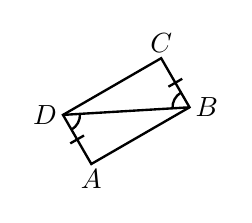
\begin{tikzpicture}

\def\len1{1.2*\lenB}

\draw[line width=0.3mm] 
(0,0) coordinate (a) --++ 
(30:\len1) coordinate (b) --++ 
(120:0.5*\len1) coordinate (c) --++ 
(210:\len1) coordinate (d) -- cycle ;  

\node[anchor=north, inner sep=2pt, rotate=0] (a-label) at (a) {$ A$};

\node[anchor=west, inner sep=2pt, rotate=0] (b-label) at (b) {$ B$}; 

\node[anchor=south, inner sep=2pt, rotate=0] (c-label) at (c) {$ C$};

\node[anchor=east, inner sep=2pt, rotate=0] (d-label) at (d) {$ D$};

\draw[line width=0.3mm] (b) -- (d);  

\coordinate (tick1) at ($(a)!0.5!(d)$) {}; 

\coordinate (tick2) at ($(c)!0.5!(b)$) {};  

\tikzset{onetick/.pic={\draw[line width=0.3mm] ($(0,0)+(0,0.07*\len1)$) -- ($(0,0)-(0,0.07*\len1)$) ; }}

\pic[rotate=-60] at (tick1) [pic type = onetick];  

\pic[rotate=-60] at (tick2) [pic type = onetick];  

\pic [draw, line width=0.3mm, angle radius=0.15*\len1] {angle=c--b--d}; 

\pic [draw, line width=0.3mm, angle radius=0.15*\len1] {angle=a--d--b}; 

\end{tikzpicture} 
%2
\item 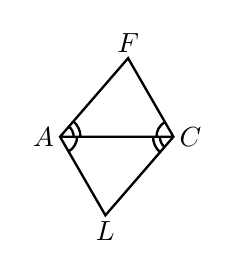
\begin{tikzpicture}

\def\len2{1.2*\lenB}

\draw[line width=0.3mm] (0,0) coordinate (a) -- (-60:0.8*\len2) coordinate (l) -- (0:\len2) coordinate (c)  --++ (120:0.8*\len2) coordinate (f) -- cycle -- (c) ;  

\node[anchor=east, inner sep=2pt, rotate=0] (a-label) at (a) {$ A$};

\node[anchor=north, inner sep=2pt, rotate=0] (l-label) at (l) {$ L$}; 

\node[anchor=west, inner sep=2pt, rotate=0] (c-label) at (c) {$ C$};

\node[anchor=south, inner sep=2pt, rotate=0] (f-label) at (f) {$ F$};

\pic [draw, line width=0.3mm, angle radius=0.15*\len2] {angle=l--a--c}; 

\pic [draw, line width=0.3mm, angle radius=0.18*\len2] {angle=a--c--l}; 

\pic [draw, line width=0.3mm, angle radius=0.12*\len2] {angle=a--c--l}; 

\pic [draw, line width=0.3mm, angle radius=0.15*\len2] {angle=f--c--a}; 

\pic [draw, line width=0.3mm, angle radius=0.12*\len2] {angle=c--a--f}; 

\pic [draw, line width=0.3mm, angle radius=0.18*\len2] {angle=c--a--f}; 

\end{tikzpicture} 
%3
\item 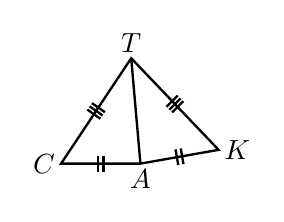
\begin{tikzpicture}

\def\len3{1.4*\lenB}

\draw[line width=0.3mm] (0,0) coordinate (a) -- (10:0.6*\len3) coordinate (k) -- (95:0.8*\len3) coordinate (t) -- (180:0.6*\len3) coordinate (c) -- cycle --  (t);  

\node[anchor=north, inner sep=2pt, rotate=0] (a-label) at (a) {$ A$};

\node[anchor=south, inner sep=2pt, rotate=0] (t-label) at (t) {$ T$}; 

\node[anchor=east, inner sep=2pt, rotate=0] (c-label) at (c) {$ C$};

\node[anchor=west, inner sep=2pt, rotate=0] (k-label) at (k) {$ K$};

\coordinate (tick1) at ($(a)!0.5!(c)$) {};  

\tikzset{twotick/.pic={\draw[line width=0.3mm] ($(-0.02*\lentick,0)+(0,0.06*\lentick)$) -- ($(-0.02*\lentick,0)-(0,0.06*\lentick)$) ($(0.02*\lentick,0)+(0,0.06*\lentick)$) -- ($(0.02*\lentick,0)-(0,0.06*\lentick)$) ; }}  
  

\tikzset{threetick/.pic={\draw[line width=0.3mm] ($(-0.03*\len3,0)+(0,0.06*\len3)$) -- ($(-0.03*\len3,0)-(0,0.06*\len3)$) ($(0,0)+(0,0.06*\len3)$) -- ($(0,0)-(0,0.06*\len3)$)  ($(0.03*\len3,0)+(0,0.06*\len3)$) -- ($(0.03*\len3,0)-(0,0.06*\len3)$) ; }}

\pic[rotate=0] at (tick1) [pic type = twotick];  

\coordinate (tick2) at ($(t)!0.5!(c)$) {};

\coordinate (tick3) at ($(a)!0.5!(k)$) {};  

\coordinate (tick4) at ($(t)!0.5!(k)$) {};

\tikzset{onetick/.pic={\draw[line width=0.3mm] ($(0,0)+(0,0.06*\len3)$) -- ($(0,0)-(0,0.06*\len3)$) ; }}

%\pic[rotate=60] at (tick2) [pic type = onetick];

\pic[rotate=55] at (tick2) [pic type = threetick];

\pic[rotate=10] at (tick3) [pic type = twotick];

\pic[rotate=-45] at (tick4) [pic type = threetick];  

\end{tikzpicture} 

\end{multicols} 
\end{enumerate}  
 


\def\figdir{/storage/emulated/0/Documents/documents/latex/1920/Grade-8/3rd/triangle-congruence-postulates/f}


\begin{enumerate}[label = \arabic*. ]
\begin{multicols}{2}
%4
\item[4. ] 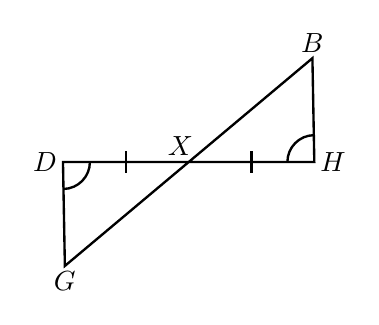
\begin{tikzpicture}

\def\len4{1.9*\lenB}

\draw[line width=0.3mm] (0,0) coordinate (x) -- (40:0.9*\len4) coordinate (b) -- (0:0.7*\len4) coordinate (h) -- (180:0.7*\len4) coordinate (d) -- (220:0.9*\len4) coordinate (g) -- cycle; 

\node[xshift=-3pt, anchor=south, inner sep=2pt, rotate=0] (x-label) at (x) {$ X$};

\node[anchor=south, inner sep=2pt, rotate=0] (b-label) at (b) {$ B$}; 

\node[anchor=west, inner sep=2pt, rotate=0] (h-label) at (h) {$ H$};

\node[anchor=east, inner sep=2pt, rotate=0] (d-label) at (d) {$ D$};

\node[anchor=north, inner sep=2pt, rotate=0] (g-label) at (g) {$ G$};

\coordinate (tick1) at ($(x)!0.5!(h)$) {}; 

\coordinate (tick2) at ($(x)!0.5!(d)$) {};  

\tikzset{onetick/.pic={\draw[line width=0.3mm] ($(0,0)+(0,0.06*\len4)$) -- ($(0,0)-(0,0.06*\len4)$) ; }}

\pic[rotate=0] at (tick1) [pic type = onetick];

\pic[rotate=0] at (tick2) [pic type = onetick];   

\pic [draw, line width=0.3mm, angle radius=0.15*\len4] {angle=b--h--x}; 

\pic [draw, line width=0.3mm, angle radius=0.15*\len4] {angle=g--d--x}; 

\end{tikzpicture} 
%5 
\item[5. ] 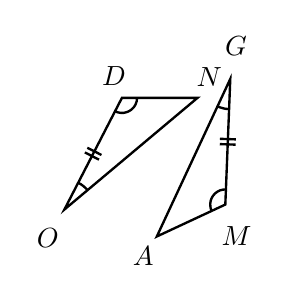
\begin{tikzpicture}

\def\len5{0.8*\lenB}

\coordinate (d) at (0,0);  

\coordinate (n) at ($(d) + (0:\len5)$); 

\coordinate (o) at ($(n) + (-140:2.3*\len5)$); 

\draw[line width=0.3mm] (d) --  (n) -- (o) -- cycle node[midway] (tick1) {} ; 

%\tikzset{twotick/.pic={\draw[line width=0.3mm] ($(-0.03*\len5,0)+(0,0.1*\len5)$) -- ($(-0.03*\len5,0)-(0,0.1*\len5)$) ($(0.03*\len5,0)+(0,0.1*\len5)$) -- ($(0.03*\len5,0)-(0,0.1*\len5)$) ; }}
\tikzset{twotick/.pic={\draw[line width=0.3mm] ($(-0.02*\lentick,0)+(0,0.06*\lentick)$) -- ($(-0.02*\lentick,0)-(0,0.06*\lentick)$) ($(0.02*\lentick,0)+(0,0.06*\lentick)$) -- ($(0.02*\lentick,0)-(0,0.06*\lentick)$) ; }}  


%\tikzset{twotick/.pic={\draw[line width=0.3mm] ($(-0.02*\len5,0)+(0,0.06*\len5)$) -- ($(-0.02*\len5,0)-(0,0.06*\len5)$) ($(0.02*\len5,0)+(0,0.06*\len5)$) -- ($(0.02*\len5,0)-(0,0.06*\len5)$) ; }}  

\pic[rotate=63] at (tick1) [pic type = twotick]; 

\pic [draw, line width=0.3mm, angle radius=0.2*\len5] {angle=o--d--n}; 

\node(d-label) at ($(d)+(110:0.25*\lenB)$) {$ D$}; 

\node(n-label) at ($(n)+(60:0.25*\lenB)$) {$ N$}; 

\node(o-label) at ($(o)-(60:0.35*\lenB)$) {$ O$}; 

\coordinate (g) at ($(n) + (30:0.5*\len5)$); 

\coordinate (a) at ($(g) + (245:2.3*\len5)$); 

\coordinate (m) at ($(a) + (25:\len5)$); 

\node(g-label) at ($(g)+(80:0.35*\lenB)$) {$ G$};

\node(m-label) at ($(m)+(-70:0.35*\lenB)$) {$ M$};

\node(a-label) at ($(a)+(235:0.25*\lenB)$) {$ A$}; 

\draw[line width=0.3mm] (g) -- (a)--(m) -- cycle node[midway] (tick2) {} ; 

\pic[rotate=88] at (tick2) [pic type = twotick];  

\pic [draw, line width=0.3mm, angle radius=0.2*\len5] {angle=g--m--a}; 

\pic [draw, line width=0.3mm, angle radius=0.4*\len5] {angle=a--g--m}; 

\pic [draw, line width=0.3mm, angle radius=0.4*\len5] {angle=n--o--d}; 

\end{tikzpicture} 

\end{multicols} 
\end{enumerate}  
 


\begin{enumerate}[label = \arabic*. ]
\begin{multicols}{3}

%1
\item $\overline{CB} \cong$ \blank \\
$\overline{BD} \cong$ \blank \\
$\angle{CBD} \cong$ \blank \\
$\triangle{CBD} \cong$ \blank \\
Postulate: \blank
%2
\item $\overline{AC} \cong$ \blank \\
$\angle{FCA} \cong$ \blank \\
$\angle{FAC} \cong$ \blank \\
$\triangle{FCA} \cong$ \blank \\
Postulate: \blank
%3
\item $\overline{AT} \cong$ \blank \\
$\overline{AC} \cong$ \blank \\
$\overline{CT} \cong$ \blank \\
$\triangle{ACT} \cong$ \blank \\
Postulate: \blank
%4
\item $\overline{DX} \cong$ \blank \\
$\angle{DXG} \cong$ \blank \\
$\angle{D} \cong$ \blank \\
$\triangle{DXG} \cong$ \blank \\
Postulate: \blank
%5
\item $\overline{DO} \cong$ \blank \\
$\angle{O} \cong$ \blank \\
$\angle{D} \cong$ \blank \\
$\triangle{DON} \cong$ \blank \\
Postulate: \blank

\end{multicols} 
\end{enumerate}   
%}}

%\input{hand-triangle-congruence-postulates-input2}
%\vspace*{1ex}
\def\figdir{/storage/emulated/0/Documents/documents/latex/1920/Grade-8/3rd/triangle-congruence-postulates/f}


%\textbf{Practice Exercises}
\textbf{Problem Set}

\vspce
A. Fill in the blanks then indicate the congruence postulate used. 

%\begin{center}
%\vspace*{2ex}
%\scalebox{1}{
%\noindent\begin{minipage}{\textwidth}
{\begin{enumerate}[label = \arabic*. ]
\begin{multicols}{3}
%1
\item 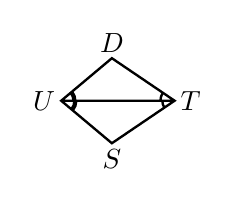
\begin{tikzpicture}

\def\len1{\lenB}

\draw[line width=0.3mm] (0,0) coordinate (u)  -- (40:0.7*\len1) coordinate (d) -- (0:1.2*\len1) coordinate (t) -- (-40:0.7*\len1) coordinate (s) -- cycle -- (t) ;  

\node[anchor=east, inner sep=2pt, rotate=0] (u-label) at (u) {$ U$}; 

\node[anchor=south, inner sep=2pt, rotate=0] (d-label) at (d) {$ D$}; 

\node[anchor=west, inner sep=2pt, rotate=0] (t-label) at (t) {$ T$}; 

\node[anchor=north, inner sep=2pt, rotate=0] (s-label) at (s) {$ S$}; 

\pic [draw, line width=0.3mm, angle radius=0.15*\len1] {angle=d--t--u}; 

\pic [draw, line width=0.3mm, angle radius=0.13*\len1] {angle=u--t--s}; 

\pic [draw, line width=0.3mm, angle radius=0.14*\len1] {angle=s--u--t}; 

\pic [draw, line width=0.3mm, angle radius=0.16*\len1] {angle=s--u--t}; 

\pic [draw, line width=0.3mm, angle radius=0.13*\len1] {angle=t--u--d}; 

\pic [draw, line width=0.3mm, angle radius=0.15*\len1] {angle=t--u--d}; 

\end{tikzpicture} 
%2
\item 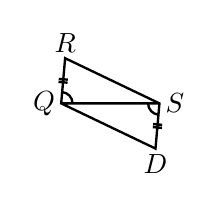
\begin{tikzpicture}

\def\len2{0.8*\lenB}

\draw[line width=0.3mm] (0,0) coordinate (q)  -- (85:0.6*\len2) coordinate (r) -- (0:1.3*\len2) coordinate (s) --++ (-95:0.6*\len2) coordinate (d) -- cycle --(s) ;  

\node[anchor=east, inner sep=2pt, rotate=0] (q-label) at (q) {$ Q$}; 

\node[anchor=south, inner sep=2pt, rotate=0] (r-label) at (r) {$ R$}; 

\node[anchor=west, inner sep=2pt, rotate=0] (s-label) at (s) {$ S$}; 

\node[anchor=north, inner sep=2pt, rotate=0] (d-label) at (d) {$ D$}; 

\coordinate (tick1) at ($(q)!0.5!(r)$) {};

\coordinate (tick2) at ($(s)!0.5!(d)$) {};  

\tikzset{twotick/.pic={\draw[line width=0.3mm] ($(-0.02*\len2, 0)+(0, 0.06*\len2)$) -- ($(-0.02*\len2, 0)-(0, 0.06*\len2)$) ($(0.02*\len2, 0)+(0, 0.06*\len2)$) -- ($(0.02*\len2, 0)-(0, 0.06*\len2)$) ; }}

\pic[rotate=85] at (tick1) [pic type = twotick];  

\pic[rotate=85] at (tick2) [pic type = twotick];   

\pic [draw, line width=0.3mm, angle radius=0.15*\len2] {angle=s--q--r}; 

\pic [draw, line width=0.3mm, angle radius=0.15*\len2] {angle=q--s--d}; 

\end{tikzpicture} 
%3
\item 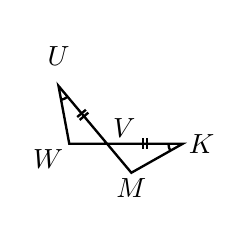
\begin{tikzpicture}%[remember picture, overlay] 

\def\len3{\lenB}

\draw[line width=0.3mm] (0,0) coordinate (v)  -- (130:0.8*\len3) coordinate (u) -- (180:0.4*\len3) coordinate (w) -- (0:0.8*\len3) coordinate (k) -- (-50:0.4*\len3) coordinate (m) -- cycle;  

\node[anchor=south west, inner sep=2pt, rotate=0] (v-label) at (v) {$ V$}; 

\node[anchor=south, inner sep=7pt, rotate=0] (u-label) at (u) {$ U$}; 

\node[anchor=north east, inner sep=2pt, rotate=0] (w-label) at (w) {$ W$}; 

\node[anchor=west, inner sep=2pt, rotate=0] (k-label) at (k) {$ K$}; 

\node[anchor=north, inner sep=2pt, rotate=0] (m-label) at (m) {$ M$}; 

\coordinate (tick1) at ($(u)!0.5!(v)$) {}; 

\coordinate (tick2) at ($(k)!0.5!(v)$) {};  

\tikzset{twotick/.pic={\draw[line width=0.3mm] ($(-0.02*\len3, 0)+(0, 0.06*\len3)$) -- ($(-0.02*\len3, 0)-(0, 0.06*\len3)$) ($(0.02*\len3, 0)+(0, 0.06*\len3)$) -- ($(0.02*\len3, 0)-(0, 0.06*\len3)$) ; }}

\pic[rotate=130] at (tick1) [pic type = twotick];

\pic[rotate=0] at (tick2) [pic type = twotick];   

\pic [draw, line width=0.3mm, angle radius=0.15*\len3] {angle=w--u--v}; 

\pic [draw, line width=0.3mm, angle radius=0.15*\len3] {angle=v--k--m}; 

\end{tikzpicture} 
%4
\item 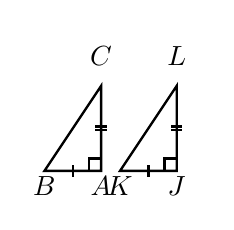
\begin{tikzpicture}

\def\len4{\lenB}

\draw[line width=0.3mm] (0,0) coordinate (a)  -- (180:0.6*\len4) coordinate (b) -- (90:0.9*\len4) coordinate (c) -- cycle;  

\node[anchor=north, inner sep=2pt, rotate=0] (a-label) at (a) {$ A$}; 

\node[anchor=north, inner sep=2pt, rotate=0] (b-label) at (b) {$ B$}; 

\node[anchor=south, inner sep=7pt, rotate=0] (c-label) at (c) {$ C$}; 

\draw[line width=0.3mm, xshift=0.8*\len4] (0,0) coordinate (j)  -- (180:0.6*\len4) coordinate (k) -- (90:0.9*\len4) coordinate (l) -- cycle;

\node[anchor=north, inner sep=2pt, rotate=0] (j-label) at (j) {$ J$}; 

\node[anchor=north, inner sep=2pt, rotate=0] (k-label) at (k) {$ K$}; 

\node[anchor=south, inner sep=7pt, rotate=0] (l-label) at (l) {$ L$}; 

\coordinate (tick1) at ($(a)!0.5!(b)$) {}; 

\coordinate (tick2) at ($(j)!0.5!(k)$) {};  

\tikzset{onetick/.pic={\draw[line width=0.3mm] ($(0,0)+(0, 0.06*\len4)$) -- ($(0,0)-(0, 0.06*\len4)$) ; }}

\pic[rotate=0] at (tick1) [pic type = onetick]; 

\pic[rotate=0] at (tick2) [pic type = onetick];   

\coordinate (tick3) at ($(a)!0.5!(c)$) {};  

\coordinate (tick4) at ($(l)!0.5!(j)$) {};  

\tikzset{twotick/.pic={\draw[line width=0.3mm] ($(-0.02*\len4, 0)+(0, 0.06*\len4)$) -- ($(-0.02*\len4, 0)-(0, 0.06*\len4)$) ($(0.02*\len4, 0)+(0, 0.06*\len4)$) -- ($(0.02*\len4, 0)-(0, 0.06*\len4)$) ; }}

\pic[rotate=90] at (tick3) [pic type = twotick];

\pic[rotate=90] at (tick4) [pic type = twotick];  

\begin{scope} [rotate=90]
\draw[line width=0.3mm] (a) rectangle ++(0.13*\len4,0.13*\len4) node[transform shape]{};
\end{scope} 

\begin{scope} [rotate=90]
\draw[line width=0.3mm] (j) rectangle ++(0.13*\len4,0.13*\len4) node[transform shape]{};
\end{scope} 

\end{tikzpicture} 
%5
\item 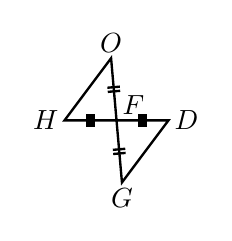
\begin{tikzpicture}

\def\len5{1.1*\lenB}

\draw[line width=0.3mm] (0,0) coordinate (f)  -- (95:0.6*\len5) coordinate (o) -- (180:0.5*\len5) coordinate (h)  -- (0:0.5*\len5) coordinate (d) -- (-85:0.6*\len5) coordinate (g) -- cycle;  

\node[anchor=south west, inner sep=2pt, rotate=0] (f-label) at (f) {$ F$};

\node[anchor=south, inner sep=2pt, rotate=0] (o-label) at (o) {$ O$};

\node[anchor=east, inner sep=2pt, rotate=0] (h-label) at (h) {$ H$};

\node[anchor=west, inner sep=2pt, rotate=0] (d-label) at (d) {$ D$};

\node[anchor=north, inner sep=2pt, rotate=0] (g-label) at (g) {$ G$};

\coordinate (tick1) at ($(o)!0.5!(f)$) {};  

\coordinate (tick2) at ($(f)!0.5!(g)$) {};  

\tikzset{twotick/.pic={\draw[line width=0.3mm] ($(-0.02*\len5, 0)+(0, 0.06*\len5)$) -- ($(-0.02*\len5, 0)-(0, 0.06*\len5)$) ($(0.02*\len5, 0)+(0, 0.06*\len5)$) -- ($(0.02*\len5, 0)-(0, 0.06*\len5)$) ; }}

\pic[rotate=95] at (tick1) [pic type = twotick]; 

\pic[rotate=95] at (tick2) [pic type = twotick];   

\coordinate (tick3) at ($(h)!0.5!(f)$) {};  

\coordinate (tick4) at ($(f)!0.5!(d)$) {};  

\tikzset{threetick/.pic={\draw[line width=0.3mm] ($(-0.03*\len5, 0)+(0, 0.06*\len5)$) -- ($(-0.03*\len5, 0)-(0, 0.06*\len5)$) ($(0,0)+(0, 0.06*\len5)$) -- ($(0,0)-(0, 0.06*\len5)$)  ($(0.03*\len5, 0)+(0, 0.06*\len5)$) -- ($(0.03*\len5, 0)-(0, 0.06*\len5)$) ; }}

\pic[rotate=0] at (tick3) [pic type = threetick]; 

\pic[rotate=0] at (tick4) [pic type = threetick];   

\end{tikzpicture} 
%6
\item 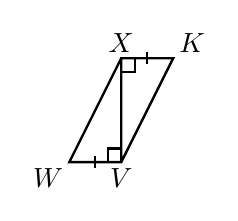
\begin{tikzpicture}

\def\len6{1.1*\lenB}

\draw[line width=0.3mm] (0,0) coordinate (v)  -- (180:0.5*\len6) coordinate (w) -- (90:\len6) coordinate (x) --++ (0:0.5*\len6) coordinate (k) -- cycle -- (x) ; 

\node[anchor=north, inner sep=2pt, rotate=0] (v-label) at (v) {$ V$};

\node[anchor=north east, inner sep=2pt, rotate=0] (w-label) at (w) {$ W$};

\node[anchor=south, inner sep=2pt, rotate=0] (x-label) at (x) {$ X$};

\node[anchor=south west, inner sep=2pt, rotate=0] (k-label) at (k) {$ K$};

\begin{scope} [rotate=90]
\draw[line width=0.3mm] (v) rectangle ++(0.13*\len6,0.13*\len6) node[transform shape]{};
\end{scope} 

\begin{scope} [rotate=-90]
\draw[line width=0.3mm] (x) rectangle ++(0.13*\len6,0.13*\len6) node[transform shape]{};
\end{scope} 

\coordinate (tick1) at ($(w)!0.5!(v)$) {};  

\coordinate (tick2) at ($(x)!0.5!(k)$) {};  

\tikzset{onetick/.pic={\draw[line width=0.3mm] ($(0,0)+(0, 0.06*\len6)$) -- ($(0,0)-(0, 0.06*\len6)$) ; }}

\pic[rotate=0] at (tick1) [pic type = onetick];

\pic[rotate=0] at (tick2) [pic type = onetick];   

\end{tikzpicture} 
%7
%\item 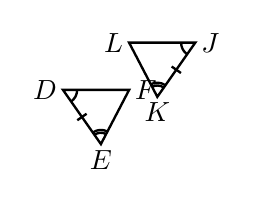
\begin{tikzpicture}

\def\len7{\lenB}

\draw[line width=0.3mm] (0,0) coordinate (d)  -- (-55:0.7*\len7) coordinate (e) -- (0:0.7*\len7) coordinate (f) -- cycle; 

\node[anchor=east, inner sep=2pt, rotate=0] (d-label) at (d) {$ D$};

\node[anchor=north, inner sep=2pt, rotate=0] (e-label) at (e) {$ E$};

\node[anchor=west, inner sep=2pt, rotate=0] (f-label) at (f) {$ F$};

\draw[line width=0.3mm, xshift=0.7*\len7, yshift=0.5*\len7, remember picture, overlay]  (0,0) coordinate (l) -- (0:0.7*\len7) coordinate (j) --++ (235:0.7*\len7) coordinate (k) -- cycle; 

\node[anchor=west, inner sep=2pt, rotate=0] (j-label) at (j) {$ J$};

\node[anchor=north, inner sep=2pt, rotate=0] (k-label) at (k) {$ K$};

\node[anchor=east, inner sep=2pt, rotate=0] (l-label) at (l) {$ L$};

\pic [draw, line width=0.3mm, angle radius=0.15*\len7] {angle=e--d--f};

\pic [draw, line width=0.3mm, angle radius=0.15*\len7] {angle=l--j--k};

\pic [draw, line width=0.3mm, angle radius=0.15*\len7] {angle=f--e--d};

\pic [draw, line width=0.3mm, angle radius=0.12*\len7] {angle=f--e--d};

\pic [draw, line width=0.3mm, angle radius=0.15*\len7] {angle=j--k--l};

\pic [draw, line width=0.3mm, angle radius=0.12*\len7] {angle=j--k--l};

\coordinate (tick1) at ($(d)!0.5!(e)$) {};  

\coordinate (tick2) at ($(j)!0.5!(k)$) {};  

\tikzset{onetick/.pic={\draw[line width=0.3mm] ($(0,0)+(0, 0.06*\len7)$) -- ($(0,0)-(0, 0.06*\len7)$) ; }}

\pic[rotate=-55] at (tick1) [pic type = onetick]; 

\pic[rotate=55] at (tick2) [pic type = onetick];   

\end{tikzpicture} 
%8
%\item 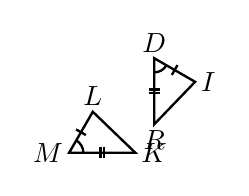
\begin{tikzpicture}

\def\len8{\lenB}

\draw[line width=0.3mm, remember picture, overlay] (0,0) coordinate (m)  -- (60:0.5*\len8) coordinate (l) -- (0:0.7*\len8) coordinate (k) -- cycle; 

\node[anchor=east, inner sep=2pt, rotate=0] (m-label) at (m) {$ M$};

\node[anchor=south, inner sep=2pt, rotate=0] (l-label) at (l) {$ L$};

\node[anchor=west, inner sep=2pt, rotate=0] (k-label) at (k) {$ K$};

\draw[line width=0.3mm, rotate=-90, xshift=-1*\len8,
yshift=0.9*\len8
] (0,0) coordinate (d)  -- (60:0.5*\len8) coordinate (i) -- (0:0.7*\len8) coordinate (r) -- cycle; 

\node[anchor=south, inner sep=2pt, rotate=0] (d-label) at (d) {$ D$};

\node[anchor=west, inner sep=2pt, rotate=0] (i-label) at (i) {$ I$};

\node[anchor=north, inner sep=2pt, rotate=0] (r-label) at (r) {$ R$};

\pic [draw, line width=0.3mm, angle radius=0.15*\len8] {angle=k--m--l}; 

\pic [draw, line width=0.3mm, angle radius=0.15*\len8] {angle=r--d--i}; 

\coordinate (tick1) at ($(l)!0.5!(m)$) {};  

\coordinate (tick2) at ($(d)!0.5!(i)$) {};  

\tikzset{onetick/.pic={\draw[line width=0.3mm] ($(0,0)+(0, 0.06*\len8)$) -- ($(0,0)-(0, 0.06*\len8)$) ; }}

\pic[rotate=60] at (tick1) [pic type = onetick];

\pic[rotate=-30] at (tick2) [pic type = onetick]; 

\coordinate (tick3) at ($(k)!0.5!(m)$) {};  

\coordinate (tick4) at ($(d)!0.5!(r)$) {};  

\tikzset{twotick/.pic={\draw[line width=0.3mm] ($(-0.02*\len8, 0)+(0, 0.06*\len8)$) -- ($(-0.02*\len8, 0)-(0, 0.06*\len8)$) ($(0.02*\len8, 0)+(0, 0.06*\len8)$) -- ($(0.02*\len8, 0)-(0, 0.06*\len8)$) ; }}

\pic[rotate=0] at (tick3) [pic type = twotick];

\pic[rotate=90] at (tick4) [pic type = twotick];    

\end{tikzpicture} 

\end{multicols} 
\end{enumerate}}
%\end{minipage}}
%\end{center}  

    
\begin{enumerate}[label = \arabic*. ]
\begin{multicols}{3}

%1
\item $\overline{TU} \cong$ \blank \\
$\angle{DUT} \cong$ \blank \\
$\angle{DTU} \cong$ \blank \\
$\triangle{DUT} \cong$ \blank \\
Postulate: \blank
%2
\item $\overline{QS} \cong$ \blank \\
$\overline{QR} \cong$ \blank \\
$\angle{RQS} \cong$ \blank \\
$\triangle{RQS} \cong$ \blank \\
Postulate: \blank
%3
\item $\overline{UV} \cong$ \blank \\
$\angle{U} \cong$ \blank \\
$\angle{UVW} \cong$ \blank \\
$\triangle{UVW} \cong$ \blank \\
Postulate: \blank
%4
\item $\overline{AB} \cong$ \blank \\
$\overline{AC} \cong$ \blank \\
$\angle{A} \cong$ \blank \\
$\triangle{ABC} \cong$ \blank \\
Postulate: \blank
%5
\item $\overline{FO} \cong$ \blank \\
$\overline{HF} \cong$ \blank \\
$\angle{HFO} \cong$ \blank \\
$\triangle{HFO} \cong$ \blank \\
Postulate: \blank
%6
\item $\overline{KX} \cong$ \blank \\
$\overline{XV} \cong$ \blank \\
$\angle{KXV} \cong$ \blank \\
$\triangle{KXV} \cong$ \blank \\
Postulate: \blank

\end{multicols} 
\end{enumerate}   
%}}



\end{frame}

% frame 3
\vertadjustb
\begin{frame} 
\begin{center}
\textbf{Triangle Congruence Postulates 
}
\end{center}

\vspce

Included angle: the angle between two sides of a triangle 

\vspce 

Included side: the side common to  two angles  of a triangle 


\vspce 

SSS (Side-Side-Side) Congruence Postulate: If the three sides of one triangle are congruent to the corresponding sides of another triangle, then the two triangles are congruent.

\vspce 

SAS (Side-Angle-Side) Congruence Postulate: 

If the two sides and an included angle of one triangle are congruent to the corresponding  two sides and included angle of another triangle, then the two triangles are congruent.

\vspce 

ASA (Angle-Side-Angle) Congruence Postulate: If two angles and the included side of one triangle are congruent to the corresponding two angles and included side of another triangle, then the two triangles are congruent. 

\vspce 

HL (Hypotenuse-Leg) Congruence Postulate: If the hypotenuse and a leg of one right triangle are congruent to the corresponding hypotenuse and side of another right triangle, then the two right triangles are congruent.



 
\def\figdir{/storage/emulated/0/Documents/documents/latex/1920/Grade-8/3rd/triangle-congruence-postulates/f}

\textbf{Practice Exercises}
%\textbf{Problem Set}

\vspce

%\begin{enumerate}[label = \Alph*. ]
%A
%\item \hspce 
A. The figures are marked with their congruent parts. Determine the other congruent parts to satisfy the condition written for each figure. 

%\begin{multicols}{2}

\begin{enumerate}[label = \arabic*. ]

\begin{multicols}{2}

%1
\item SAS \\
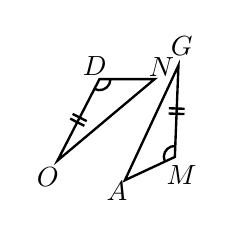
\begin{tikzpicture}

\coordinate (d) at (0,0);  

\coordinate (n) at ($(d) + (0:\lenA)$); 

\coordinate (o) at ($(n) + (-140:2.3*\lenA)$); 

\draw[line width=0.3mm] (d) --  (n) -- (o) -- cycle node[midway] (tick1) {} ; 

%\tikzset{twotick/.pic={\draw[line width=0.3mm] ($(-0.08,0)+(0,0.1*\lenA)$) -- ($(-0.08,0)-(0,0.1*\lenA)$) ($(0.08,0)+(0,0.1*\lenA)$) -- ($(0.08,0)-(0,0.1*\lenA)$) ; }}

\tikzset{twotick/.pic={\draw[line width=0.3mm] ($(-0.02*\lentick,0)+(0,0.06*\lentick)$) -- ($(-0.02*\lentick,0)-(0,0.06*\lentick)$) ($(0.02*\lentick,0)+(0,0.06*\lentick)$) -- ($(0.02*\lentick,0)-(0,0.06*\lentick)$) ; }}  

%\tikzset{twotick/.pic={\draw[line width=0.3mm] ($(-0.02*\lentick)+(0,0.06*\lentick)$) -- ($(-0.02*\lentick,0)-(0,0.06*\lentick)$) ($(0.02*\lentick,0)+(0,0.06*\lentick)$) -- ($(0.02*\lentick,0)-(0,0.06*\lentick)$) ; }}  


\pic[rotate=63] at (tick1) [pic type = twotick]; 

\pic [draw, line width=0.3mm, angle radius=0.2*\lenA] {angle=o--d--n}; 

\node(d-label) at ($(d)+(110:0.25*\lenA)$) {$ D$}; 

\node(n-label) at ($(n)+(60:0.25*\lenA)$) {$ N$}; 

\node(o-label) at ($(o)-(60:0.35*\lenA)$) {$ O$}; 

\coordinate (g) at ($(n) + (30:0.5*\lenA)$); 

\coordinate (a) at ($(g) + (245:2.3*\lenA)$); 

\coordinate (m) at ($(a) + (25:\lenA)$); 

\node(g-label) at ($(g)+(80:0.35*\lenA)$) {$ G$};

\node(m-label) at ($(m)+(-70:0.35*\lenA)$) {$ M$};

\node(a-label) at ($(a)+(235:0.25*\lenA)$) {$ A$}; 

\draw[line width=0.3mm] (g) -- (a)--(m) -- cycle node[midway] (tick2) {} ; 

\pic[rotate=88] at (tick2) [pic type = twotick];  

\pic [draw, line width=0.3mm, angle radius=0.2*\lenA] {angle=g--m--a}; 

\end{tikzpicture} 

\vspace*{3ex} 
%2
\item[2. ] SSS\\
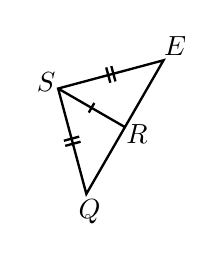
\begin{tikzpicture}

\coordinate (s) at (0,0);  

\coordinate (r) at ($(s) + (-30:1.4*\lenA)$); 

\coordinate (q) at ($(r)!1!90:(s)$); 

\coordinate (e) at ($(r)!1!-90:(s)$); 

\draw[line width=0.3mm] (s)--(q) node[midway] (tick2) {} --(e) -- cycle node[midway] (tick3) {}  (s) --(r) node[midway] (tick1) {} ; 

\node(s-label) at ($(s)+(150:0.25*\lenA)$) {$ S$}; 

\node(q-label) at ($(q)+(280:0.33*\lenA)$) {$ Q$}; 

\node(r-label) at ($(r)+(-30:0.25*\lenA)$) {$ R$}; 

\node(e-label) at ($(e)+(50:0.33*\lenA)$) {$ E$}; 

\tikzset{onetick/.pic={\draw[line width=0.3mm] ($(0,0)+(0,0.1*\lenA)$) -- ($(0,0)-(0,0.1*\lenA)$) ; }}

\pic[rotate=-30] at (tick1) [pic type = onetick]; 

%\tikzset{twotick/.pic={\draw[line width=0.3mm] ($(-0.08,0)+(0,0.1*\lenA)$) -- ($(-0.08,0)-(0,0.1*\lenA)$) ($(0.08,0)+(0,0.1*\lenA)$) -- ($(0.08,0)-(0,0.1*\lenA)$) ; }}

%\tikzset{twotick/.pic={\draw[line width=0.3mm] ($(-0.02*\lenA,0)+(0,0.06*\lenA)$) -- ($(-0.02*\lenA,0)-(0,0.06*\lenA)$) ($(0.02*\lenA,0)+(0,0.06*\lenA)$) -- ($(0.02*\lenA,0)-(0,0.06*\lenA)$) ; }}  

\tikzset{twotick/.pic={\draw[line width=0.3mm] ($(-0.02*\lentick,0)+(0,0.06*\lentick)$) -- ($(-0.02*\lentick,0)-(0,0.06*\lentick)$) ($(0.02*\lentick,0)+(0,0.06*\lentick)$) -- ($(0.02*\lentick,0)-(0,0.06*\lentick)$) ; }}  



\pic[rotate=105] at (tick2) [pic type = twotick];  

\pic[rotate=15] at (tick3) [pic type = twotick];  

\end{tikzpicture} 
 %\\[-1ex]

\end{multicols} 
\end{enumerate} 

\vspace*{-6ex}

\begin{enumerate}[label = \arabic*. ]
\begin{multicols}{3}
%3
\item[3. ] SSS\\
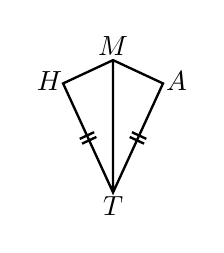
\begin{tikzpicture}

\coordinate (m) at (0,0); 

\coordinate (a) at ($(m) + (-25:\lenA)$); 

\coordinate (h) at ($(m) + (205:\lenA)$); 

\coordinate (t) at ($(m) + (-90:2.4*\lenA)$); 

\node(m-label) at ($(m)+(90:0.25*\lenA)$) {$ M$};

\node(a-label) at ($(a)+(10:0.25*\lenA)$) {$ A$}; 

\node(t-label) at ($(t)+(-90:0.25*\lenA)$) {$ T$};

\node(h-label) at ($(h)+(170:0.25*\lenA)$) {$ H$};

\draw[line width=0.3mm] (m)--(a) -- (t) node[midway] (tick1) {} --(h) node[midway] (tick2) {} -- cycle  (m)--(t); 

%\tikzset{twotick/.pic={\draw[line width=0.3mm] ($(-0.08,0)+(0,0.1*\lenA)$) -- ($(-0.08,0)-(0,0.1*\lenA)$) ($(0.08,0)+(0,0.1*\lenA)$) -- ($(0.08,0)-(0,0.1*\lenA)$) ; }}

%\tikzset{twotick/.pic={\draw[line width=0.3mm] ($(-0.02*\lenA,0)+(0,0.06*\lenA)$) -- ($(-0.02*\lenA,0)-(0,0.06*\lenA)$) ($(0.02*\lenA,0)+(0,0.06*\lenA)$) -- ($(0.02*\lenA,0)-(0,0.06*\lenA)$) ; }}  

\tikzset{twotick/.pic={\draw[line width=0.3mm] ($(-0.02*\lentick,0)+(0,0.06*\lentick)$) -- ($(-0.02*\lentick,0)-(0,0.06*\lentick)$) ($(0.02*\lentick,0)+(0,0.06*\lentick)$) -- ($(0.02*\lentick,0)-(0,0.06*\lentick)$) ; }}  



\pic[rotate=65] at (tick1) [pic type = twotick]; 

\pic[rotate=115] at (tick2) [pic type = twotick]; 

\end{tikzpicture} 


%4
\item[4. ] ASA\\
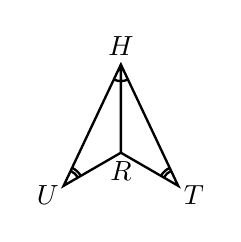
\begin{tikzpicture}

\coordinate (h) at (0,0); 

\coordinate (r) at ($(h) + (-90:1.6*\lenA)$); 

\coordinate (t) at ($(r) + (-30:1.2*\lenA)$); 

\coordinate (u) at ($(r) + (210:1.2*\lenA)$); 

\node(r-label) at ($(r)+(-90:0.33*\lenA)$) {$ R$}; 

\node(t-label) at ($(t)+(-30:0.33*\lenA)$) {$ T$}; 

\node(h-label) at ($(h)+(90:0.33*\lenA)$) {$ H$}; 

\node(u-label) at ($(u)+(210:0.33*\lenA)$) {$ U$}; 

\draw[line width=0.3mm] (h)--(t) --(r) --(u) -- cycle (h) --(r) ; 

\pic [draw, line width=0.3mm, angle radius=0.3*\lenA] {angle=u--h--r}; 

\pic [draw, line width=0.3mm, angle radius=0.3*\lenA] {angle=r--h--t}; 

\pic [draw, line width=0.3mm, angle radius=0.3*\lenA] {angle=r--u--h}; 

\pic [draw, line width=0.3mm, angle radius=0.36*\lenA] {angle=r--u--h}; 

\pic [draw, line width=0.3mm, angle radius=0.3*\lenA] {angle=h--t--r}; 

\pic [draw, line width=0.3mm, angle radius=0.36*\lenA] {angle=h--t--r}; 

\end{tikzpicture} 


%5
\item[5. ] SAS\\
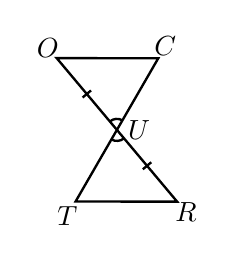
\begin{tikzpicture}

\coordinate (u) at (0,0); 

\coordinate (c) at ($(u) + (60:1.5*\lenA)$); 

\coordinate (t) at ($(u) - (60:1.5*\lenA)$); 

\coordinate (o) at ($(u) + (130:1.7*\lenA)$); 

\coordinate (r) at ($(u) - (130:1.7*\lenA)$); 

\node(u-label) at ($(u)+(0:0.4*\lenA)$) {$ U$};

\node(c-label) at ($(c)+(60:0.25*\lenA)$) {$ C$};

\node(o-label) at ($(o)+(130:0.25*\lenA)$) {$ O$};

\node(t-label) at ($(t)-(60:0.3*\lenA)$) {$ T$};

\node(r-label) at ($(r)-(130:0.25*\lenA)$) {$ R$}; 

\draw[line width=0.3mm] (u)--(o) node[midway] (tick1) {} --(c)--(t)--(r)--cycle node[midway] (tick2) {} ; 

\tikzset{onetick/.pic={\draw[line width=0.3mm] ($(0,0)+(0,0.1*\lenA)$) -- ($(0,0)-(0,0.1*\lenA)$) ; }}

\pic[rotate=-50] at (tick1) [pic type = onetick]; 

\pic[rotate=-50] at (tick2) [pic type = onetick]; 

\pic [draw, line width=0.3mm, angle radius=0.2*\lenA] {angle=c--u--o}; 

\pic [draw, line width=0.3mm, angle radius=0.2*\lenA] {angle=t--u--r}; 

\end{tikzpicture} 



\end{multicols} 

\end{enumerate} 

B. Fill in the blanks then indicate the congruence postulate used. 

\begin{enumerate}[label = \arabic*. ]
\begin{multicols}{3}
%1
\item 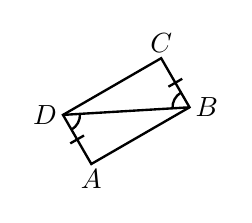
\begin{tikzpicture}

\def\len1{1.2*\lenB}

\draw[line width=0.3mm] 
(0,0) coordinate (a) --++ 
(30:\len1) coordinate (b) --++ 
(120:0.5*\len1) coordinate (c) --++ 
(210:\len1) coordinate (d) -- cycle ;  

\node[anchor=north, inner sep=2pt, rotate=0] (a-label) at (a) {$ A$};

\node[anchor=west, inner sep=2pt, rotate=0] (b-label) at (b) {$ B$}; 

\node[anchor=south, inner sep=2pt, rotate=0] (c-label) at (c) {$ C$};

\node[anchor=east, inner sep=2pt, rotate=0] (d-label) at (d) {$ D$};

\draw[line width=0.3mm] (b) -- (d);  

\coordinate (tick1) at ($(a)!0.5!(d)$) {}; 

\coordinate (tick2) at ($(c)!0.5!(b)$) {};  

\tikzset{onetick/.pic={\draw[line width=0.3mm] ($(0,0)+(0,0.07*\len1)$) -- ($(0,0)-(0,0.07*\len1)$) ; }}

\pic[rotate=-60] at (tick1) [pic type = onetick];  

\pic[rotate=-60] at (tick2) [pic type = onetick];  

\pic [draw, line width=0.3mm, angle radius=0.15*\len1] {angle=c--b--d}; 

\pic [draw, line width=0.3mm, angle radius=0.15*\len1] {angle=a--d--b}; 

\end{tikzpicture} 
%2
\item 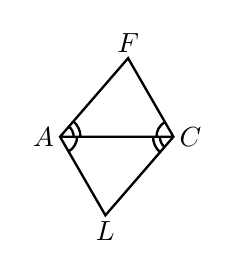
\begin{tikzpicture}

\def\len2{1.2*\lenB}

\draw[line width=0.3mm] (0,0) coordinate (a) -- (-60:0.8*\len2) coordinate (l) -- (0:\len2) coordinate (c)  --++ (120:0.8*\len2) coordinate (f) -- cycle -- (c) ;  

\node[anchor=east, inner sep=2pt, rotate=0] (a-label) at (a) {$ A$};

\node[anchor=north, inner sep=2pt, rotate=0] (l-label) at (l) {$ L$}; 

\node[anchor=west, inner sep=2pt, rotate=0] (c-label) at (c) {$ C$};

\node[anchor=south, inner sep=2pt, rotate=0] (f-label) at (f) {$ F$};

\pic [draw, line width=0.3mm, angle radius=0.15*\len2] {angle=l--a--c}; 

\pic [draw, line width=0.3mm, angle radius=0.18*\len2] {angle=a--c--l}; 

\pic [draw, line width=0.3mm, angle radius=0.12*\len2] {angle=a--c--l}; 

\pic [draw, line width=0.3mm, angle radius=0.15*\len2] {angle=f--c--a}; 

\pic [draw, line width=0.3mm, angle radius=0.12*\len2] {angle=c--a--f}; 

\pic [draw, line width=0.3mm, angle radius=0.18*\len2] {angle=c--a--f}; 

\end{tikzpicture} 
%3
\item 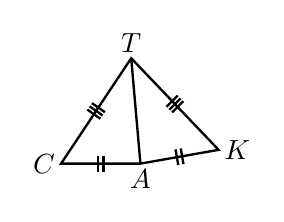
\begin{tikzpicture}

\def\len3{1.4*\lenB}

\draw[line width=0.3mm] (0,0) coordinate (a) -- (10:0.6*\len3) coordinate (k) -- (95:0.8*\len3) coordinate (t) -- (180:0.6*\len3) coordinate (c) -- cycle --  (t);  

\node[anchor=north, inner sep=2pt, rotate=0] (a-label) at (a) {$ A$};

\node[anchor=south, inner sep=2pt, rotate=0] (t-label) at (t) {$ T$}; 

\node[anchor=east, inner sep=2pt, rotate=0] (c-label) at (c) {$ C$};

\node[anchor=west, inner sep=2pt, rotate=0] (k-label) at (k) {$ K$};

\coordinate (tick1) at ($(a)!0.5!(c)$) {};  

\tikzset{twotick/.pic={\draw[line width=0.3mm] ($(-0.02*\lentick,0)+(0,0.06*\lentick)$) -- ($(-0.02*\lentick,0)-(0,0.06*\lentick)$) ($(0.02*\lentick,0)+(0,0.06*\lentick)$) -- ($(0.02*\lentick,0)-(0,0.06*\lentick)$) ; }}  
  

\tikzset{threetick/.pic={\draw[line width=0.3mm] ($(-0.03*\len3,0)+(0,0.06*\len3)$) -- ($(-0.03*\len3,0)-(0,0.06*\len3)$) ($(0,0)+(0,0.06*\len3)$) -- ($(0,0)-(0,0.06*\len3)$)  ($(0.03*\len3,0)+(0,0.06*\len3)$) -- ($(0.03*\len3,0)-(0,0.06*\len3)$) ; }}

\pic[rotate=0] at (tick1) [pic type = twotick];  

\coordinate (tick2) at ($(t)!0.5!(c)$) {};

\coordinate (tick3) at ($(a)!0.5!(k)$) {};  

\coordinate (tick4) at ($(t)!0.5!(k)$) {};

\tikzset{onetick/.pic={\draw[line width=0.3mm] ($(0,0)+(0,0.06*\len3)$) -- ($(0,0)-(0,0.06*\len3)$) ; }}

%\pic[rotate=60] at (tick2) [pic type = onetick];

\pic[rotate=55] at (tick2) [pic type = threetick];

\pic[rotate=10] at (tick3) [pic type = twotick];

\pic[rotate=-45] at (tick4) [pic type = threetick];  

\end{tikzpicture} 

\end{multicols} 
\end{enumerate}  
 


%\def\figdir{/storage/emulated/0/Documents/documents/latex/1920/Grade-8/3rd/triangle-congruence-postulates/f}


\begin{enumerate}[label = \arabic*. ]
\begin{multicols}{2}
%4
\item[4. ] 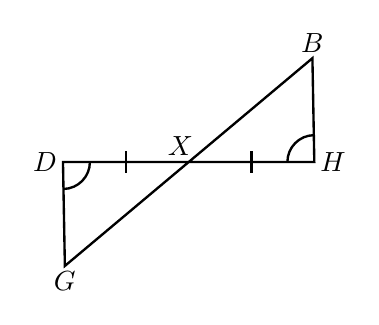
\begin{tikzpicture}

\def\len4{1.9*\lenB}

\draw[line width=0.3mm] (0,0) coordinate (x) -- (40:0.9*\len4) coordinate (b) -- (0:0.7*\len4) coordinate (h) -- (180:0.7*\len4) coordinate (d) -- (220:0.9*\len4) coordinate (g) -- cycle; 

\node[xshift=-3pt, anchor=south, inner sep=2pt, rotate=0] (x-label) at (x) {$ X$};

\node[anchor=south, inner sep=2pt, rotate=0] (b-label) at (b) {$ B$}; 

\node[anchor=west, inner sep=2pt, rotate=0] (h-label) at (h) {$ H$};

\node[anchor=east, inner sep=2pt, rotate=0] (d-label) at (d) {$ D$};

\node[anchor=north, inner sep=2pt, rotate=0] (g-label) at (g) {$ G$};

\coordinate (tick1) at ($(x)!0.5!(h)$) {}; 

\coordinate (tick2) at ($(x)!0.5!(d)$) {};  

\tikzset{onetick/.pic={\draw[line width=0.3mm] ($(0,0)+(0,0.06*\len4)$) -- ($(0,0)-(0,0.06*\len4)$) ; }}

\pic[rotate=0] at (tick1) [pic type = onetick];

\pic[rotate=0] at (tick2) [pic type = onetick];   

\pic [draw, line width=0.3mm, angle radius=0.15*\len4] {angle=b--h--x}; 

\pic [draw, line width=0.3mm, angle radius=0.15*\len4] {angle=g--d--x}; 

\end{tikzpicture} 
%5 
\item[5. ] 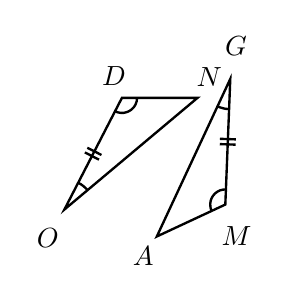
\begin{tikzpicture}

\def\len5{0.8*\lenB}

\coordinate (d) at (0,0);  

\coordinate (n) at ($(d) + (0:\len5)$); 

\coordinate (o) at ($(n) + (-140:2.3*\len5)$); 

\draw[line width=0.3mm] (d) --  (n) -- (o) -- cycle node[midway] (tick1) {} ; 

%\tikzset{twotick/.pic={\draw[line width=0.3mm] ($(-0.03*\len5,0)+(0,0.1*\len5)$) -- ($(-0.03*\len5,0)-(0,0.1*\len5)$) ($(0.03*\len5,0)+(0,0.1*\len5)$) -- ($(0.03*\len5,0)-(0,0.1*\len5)$) ; }}
\tikzset{twotick/.pic={\draw[line width=0.3mm] ($(-0.02*\lentick,0)+(0,0.06*\lentick)$) -- ($(-0.02*\lentick,0)-(0,0.06*\lentick)$) ($(0.02*\lentick,0)+(0,0.06*\lentick)$) -- ($(0.02*\lentick,0)-(0,0.06*\lentick)$) ; }}  


%\tikzset{twotick/.pic={\draw[line width=0.3mm] ($(-0.02*\len5,0)+(0,0.06*\len5)$) -- ($(-0.02*\len5,0)-(0,0.06*\len5)$) ($(0.02*\len5,0)+(0,0.06*\len5)$) -- ($(0.02*\len5,0)-(0,0.06*\len5)$) ; }}  

\pic[rotate=63] at (tick1) [pic type = twotick]; 

\pic [draw, line width=0.3mm, angle radius=0.2*\len5] {angle=o--d--n}; 

\node(d-label) at ($(d)+(110:0.25*\lenB)$) {$ D$}; 

\node(n-label) at ($(n)+(60:0.25*\lenB)$) {$ N$}; 

\node(o-label) at ($(o)-(60:0.35*\lenB)$) {$ O$}; 

\coordinate (g) at ($(n) + (30:0.5*\len5)$); 

\coordinate (a) at ($(g) + (245:2.3*\len5)$); 

\coordinate (m) at ($(a) + (25:\len5)$); 

\node(g-label) at ($(g)+(80:0.35*\lenB)$) {$ G$};

\node(m-label) at ($(m)+(-70:0.35*\lenB)$) {$ M$};

\node(a-label) at ($(a)+(235:0.25*\lenB)$) {$ A$}; 

\draw[line width=0.3mm] (g) -- (a)--(m) -- cycle node[midway] (tick2) {} ; 

\pic[rotate=88] at (tick2) [pic type = twotick];  

\pic [draw, line width=0.3mm, angle radius=0.2*\len5] {angle=g--m--a}; 

\pic [draw, line width=0.3mm, angle radius=0.4*\len5] {angle=a--g--m}; 

\pic [draw, line width=0.3mm, angle radius=0.4*\len5] {angle=n--o--d}; 

\end{tikzpicture} 

\end{multicols} 
\end{enumerate}  
 


\begin{enumerate}[label = \arabic*. ]
\begin{multicols}{3}

%1
\item $\overline{CB} \cong$ \blank \\
$\overline{BD} \cong$ \blank \\
$\angle{CBD} \cong$ \blank \\
$\triangle{CBD} \cong$ \blank \\
Postulate: \blank
%2
\item $\overline{AC} \cong$ \blank \\
$\angle{FCA} \cong$ \blank \\
$\angle{FAC} \cong$ \blank \\
$\triangle{FCA} \cong$ \blank \\
Postulate: \blank
%3
\item $\overline{AT} \cong$ \blank \\
$\overline{AC} \cong$ \blank \\
$\overline{CT} \cong$ \blank \\
$\triangle{ACT} \cong$ \blank \\
Postulate: \blank
%4
\item $\overline{DX} \cong$ \blank \\
$\angle{DXG} \cong$ \blank \\
$\angle{D} \cong$ \blank \\
$\triangle{DXG} \cong$ \blank \\
Postulate: \blank
%5
\item $\overline{DO} \cong$ \blank \\
$\angle{O} \cong$ \blank \\
$\angle{D} \cong$ \blank \\
$\triangle{DON} \cong$ \blank \\
Postulate: \blank

\end{multicols} 
\end{enumerate}   
%}}

%\vspace*{1ex}
%\def\figdir{/storage/emulated/0/Documents/documents/latex/1920/Grade-8/3rd/triangle-congruence-postulates/f}


%\textbf{Practice Exercises}
\textbf{Problem Set}

\vspce
A. Fill in the blanks then indicate the congruence postulate used. 

%\begin{center}
%\vspace*{2ex}
%\scalebox{1}{
%\noindent\begin{minipage}{\textwidth}
{\begin{enumerate}[label = \arabic*. ]
\begin{multicols}{3}
%1
\item 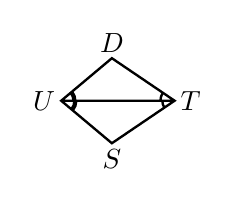
\begin{tikzpicture}

\def\len1{\lenB}

\draw[line width=0.3mm] (0,0) coordinate (u)  -- (40:0.7*\len1) coordinate (d) -- (0:1.2*\len1) coordinate (t) -- (-40:0.7*\len1) coordinate (s) -- cycle -- (t) ;  

\node[anchor=east, inner sep=2pt, rotate=0] (u-label) at (u) {$ U$}; 

\node[anchor=south, inner sep=2pt, rotate=0] (d-label) at (d) {$ D$}; 

\node[anchor=west, inner sep=2pt, rotate=0] (t-label) at (t) {$ T$}; 

\node[anchor=north, inner sep=2pt, rotate=0] (s-label) at (s) {$ S$}; 

\pic [draw, line width=0.3mm, angle radius=0.15*\len1] {angle=d--t--u}; 

\pic [draw, line width=0.3mm, angle radius=0.13*\len1] {angle=u--t--s}; 

\pic [draw, line width=0.3mm, angle radius=0.14*\len1] {angle=s--u--t}; 

\pic [draw, line width=0.3mm, angle radius=0.16*\len1] {angle=s--u--t}; 

\pic [draw, line width=0.3mm, angle radius=0.13*\len1] {angle=t--u--d}; 

\pic [draw, line width=0.3mm, angle radius=0.15*\len1] {angle=t--u--d}; 

\end{tikzpicture} 
%2
\item 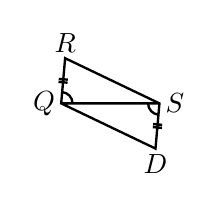
\begin{tikzpicture}

\def\len2{0.8*\lenB}

\draw[line width=0.3mm] (0,0) coordinate (q)  -- (85:0.6*\len2) coordinate (r) -- (0:1.3*\len2) coordinate (s) --++ (-95:0.6*\len2) coordinate (d) -- cycle --(s) ;  

\node[anchor=east, inner sep=2pt, rotate=0] (q-label) at (q) {$ Q$}; 

\node[anchor=south, inner sep=2pt, rotate=0] (r-label) at (r) {$ R$}; 

\node[anchor=west, inner sep=2pt, rotate=0] (s-label) at (s) {$ S$}; 

\node[anchor=north, inner sep=2pt, rotate=0] (d-label) at (d) {$ D$}; 

\coordinate (tick1) at ($(q)!0.5!(r)$) {};

\coordinate (tick2) at ($(s)!0.5!(d)$) {};  

\tikzset{twotick/.pic={\draw[line width=0.3mm] ($(-0.02*\len2, 0)+(0, 0.06*\len2)$) -- ($(-0.02*\len2, 0)-(0, 0.06*\len2)$) ($(0.02*\len2, 0)+(0, 0.06*\len2)$) -- ($(0.02*\len2, 0)-(0, 0.06*\len2)$) ; }}

\pic[rotate=85] at (tick1) [pic type = twotick];  

\pic[rotate=85] at (tick2) [pic type = twotick];   

\pic [draw, line width=0.3mm, angle radius=0.15*\len2] {angle=s--q--r}; 

\pic [draw, line width=0.3mm, angle radius=0.15*\len2] {angle=q--s--d}; 

\end{tikzpicture} 
%3
\item 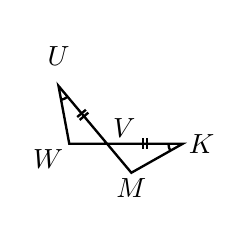
\begin{tikzpicture}%[remember picture, overlay] 

\def\len3{\lenB}

\draw[line width=0.3mm] (0,0) coordinate (v)  -- (130:0.8*\len3) coordinate (u) -- (180:0.4*\len3) coordinate (w) -- (0:0.8*\len3) coordinate (k) -- (-50:0.4*\len3) coordinate (m) -- cycle;  

\node[anchor=south west, inner sep=2pt, rotate=0] (v-label) at (v) {$ V$}; 

\node[anchor=south, inner sep=7pt, rotate=0] (u-label) at (u) {$ U$}; 

\node[anchor=north east, inner sep=2pt, rotate=0] (w-label) at (w) {$ W$}; 

\node[anchor=west, inner sep=2pt, rotate=0] (k-label) at (k) {$ K$}; 

\node[anchor=north, inner sep=2pt, rotate=0] (m-label) at (m) {$ M$}; 

\coordinate (tick1) at ($(u)!0.5!(v)$) {}; 

\coordinate (tick2) at ($(k)!0.5!(v)$) {};  

\tikzset{twotick/.pic={\draw[line width=0.3mm] ($(-0.02*\len3, 0)+(0, 0.06*\len3)$) -- ($(-0.02*\len3, 0)-(0, 0.06*\len3)$) ($(0.02*\len3, 0)+(0, 0.06*\len3)$) -- ($(0.02*\len3, 0)-(0, 0.06*\len3)$) ; }}

\pic[rotate=130] at (tick1) [pic type = twotick];

\pic[rotate=0] at (tick2) [pic type = twotick];   

\pic [draw, line width=0.3mm, angle radius=0.15*\len3] {angle=w--u--v}; 

\pic [draw, line width=0.3mm, angle radius=0.15*\len3] {angle=v--k--m}; 

\end{tikzpicture} 
%4
\item 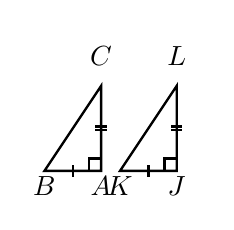
\begin{tikzpicture}

\def\len4{\lenB}

\draw[line width=0.3mm] (0,0) coordinate (a)  -- (180:0.6*\len4) coordinate (b) -- (90:0.9*\len4) coordinate (c) -- cycle;  

\node[anchor=north, inner sep=2pt, rotate=0] (a-label) at (a) {$ A$}; 

\node[anchor=north, inner sep=2pt, rotate=0] (b-label) at (b) {$ B$}; 

\node[anchor=south, inner sep=7pt, rotate=0] (c-label) at (c) {$ C$}; 

\draw[line width=0.3mm, xshift=0.8*\len4] (0,0) coordinate (j)  -- (180:0.6*\len4) coordinate (k) -- (90:0.9*\len4) coordinate (l) -- cycle;

\node[anchor=north, inner sep=2pt, rotate=0] (j-label) at (j) {$ J$}; 

\node[anchor=north, inner sep=2pt, rotate=0] (k-label) at (k) {$ K$}; 

\node[anchor=south, inner sep=7pt, rotate=0] (l-label) at (l) {$ L$}; 

\coordinate (tick1) at ($(a)!0.5!(b)$) {}; 

\coordinate (tick2) at ($(j)!0.5!(k)$) {};  

\tikzset{onetick/.pic={\draw[line width=0.3mm] ($(0,0)+(0, 0.06*\len4)$) -- ($(0,0)-(0, 0.06*\len4)$) ; }}

\pic[rotate=0] at (tick1) [pic type = onetick]; 

\pic[rotate=0] at (tick2) [pic type = onetick];   

\coordinate (tick3) at ($(a)!0.5!(c)$) {};  

\coordinate (tick4) at ($(l)!0.5!(j)$) {};  

\tikzset{twotick/.pic={\draw[line width=0.3mm] ($(-0.02*\len4, 0)+(0, 0.06*\len4)$) -- ($(-0.02*\len4, 0)-(0, 0.06*\len4)$) ($(0.02*\len4, 0)+(0, 0.06*\len4)$) -- ($(0.02*\len4, 0)-(0, 0.06*\len4)$) ; }}

\pic[rotate=90] at (tick3) [pic type = twotick];

\pic[rotate=90] at (tick4) [pic type = twotick];  

\begin{scope} [rotate=90]
\draw[line width=0.3mm] (a) rectangle ++(0.13*\len4,0.13*\len4) node[transform shape]{};
\end{scope} 

\begin{scope} [rotate=90]
\draw[line width=0.3mm] (j) rectangle ++(0.13*\len4,0.13*\len4) node[transform shape]{};
\end{scope} 

\end{tikzpicture} 
%5
\item \begin{tikzpicture}

\def\len5{1.1*\lenB}

\draw[line width=0.3mm] (0,0) coordinate (f)  -- (95:0.6*\len5) coordinate (o) -- (180:0.5*\len5) coordinate (h)  -- (0:0.5*\len5) coordinate (d) -- (-85:0.6*\len5) coordinate (g) -- cycle;  

\node[anchor=south west, inner sep=2pt, rotate=0] (f-label) at (f) {$ F$};

\node[anchor=south, inner sep=2pt, rotate=0] (o-label) at (o) {$ O$};

\node[anchor=east, inner sep=2pt, rotate=0] (h-label) at (h) {$ H$};

\node[anchor=west, inner sep=2pt, rotate=0] (d-label) at (d) {$ D$};

\node[anchor=north, inner sep=2pt, rotate=0] (g-label) at (g) {$ G$};

\coordinate (tick1) at ($(o)!0.5!(f)$) {};  

\coordinate (tick2) at ($(f)!0.5!(g)$) {};  

\tikzset{twotick/.pic={\draw[line width=0.3mm] ($(-0.02*\len5, 0)+(0, 0.06*\len5)$) -- ($(-0.02*\len5, 0)-(0, 0.06*\len5)$) ($(0.02*\len5, 0)+(0, 0.06*\len5)$) -- ($(0.02*\len5, 0)-(0, 0.06*\len5)$) ; }}

\pic[rotate=95] at (tick1) [pic type = twotick]; 

\pic[rotate=95] at (tick2) [pic type = twotick];   

\coordinate (tick3) at ($(h)!0.5!(f)$) {};  

\coordinate (tick4) at ($(f)!0.5!(d)$) {};  

\tikzset{threetick/.pic={\draw[line width=0.3mm] ($(-0.03*\len5, 0)+(0, 0.06*\len5)$) -- ($(-0.03*\len5, 0)-(0, 0.06*\len5)$) ($(0,0)+(0, 0.06*\len5)$) -- ($(0,0)-(0, 0.06*\len5)$)  ($(0.03*\len5, 0)+(0, 0.06*\len5)$) -- ($(0.03*\len5, 0)-(0, 0.06*\len5)$) ; }}

\pic[rotate=0] at (tick3) [pic type = threetick]; 

\pic[rotate=0] at (tick4) [pic type = threetick];   

\end{tikzpicture} 
%6
\item \begin{tikzpicture}

\def\len6{1.1*\lenB}

\draw[line width=0.3mm] (0,0) coordinate (v)  -- (180:0.5*\len6) coordinate (w) -- (90:\len6) coordinate (x) --++ (0:0.5*\len6) coordinate (k) -- cycle -- (x) ; 

\node[anchor=north, inner sep=2pt, rotate=0] (v-label) at (v) {$ V$};

\node[anchor=north east, inner sep=2pt, rotate=0] (w-label) at (w) {$ W$};

\node[anchor=south, inner sep=2pt, rotate=0] (x-label) at (x) {$ X$};

\node[anchor=south west, inner sep=2pt, rotate=0] (k-label) at (k) {$ K$};

\begin{scope} [rotate=90]
\draw[line width=0.3mm] (v) rectangle ++(0.13*\len6,0.13*\len6) node[transform shape]{};
\end{scope} 

\begin{scope} [rotate=-90]
\draw[line width=0.3mm] (x) rectangle ++(0.13*\len6,0.13*\len6) node[transform shape]{};
\end{scope} 

\coordinate (tick1) at ($(w)!0.5!(v)$) {};  

\coordinate (tick2) at ($(x)!0.5!(k)$) {};  

\tikzset{onetick/.pic={\draw[line width=0.3mm] ($(0,0)+(0, 0.06*\len6)$) -- ($(0,0)-(0, 0.06*\len6)$) ; }}

\pic[rotate=0] at (tick1) [pic type = onetick];

\pic[rotate=0] at (tick2) [pic type = onetick];   

\end{tikzpicture} 
%7
%\item \begin{tikzpicture}

\def\len7{\lenB}

\draw[line width=0.3mm] (0,0) coordinate (d)  -- (-55:0.7*\len7) coordinate (e) -- (0:0.7*\len7) coordinate (f) -- cycle; 

\node[anchor=east, inner sep=2pt, rotate=0] (d-label) at (d) {$ D$};

\node[anchor=north, inner sep=2pt, rotate=0] (e-label) at (e) {$ E$};

\node[anchor=west, inner sep=2pt, rotate=0] (f-label) at (f) {$ F$};

\draw[line width=0.3mm, xshift=0.7*\len7, yshift=0.5*\len7, remember picture, overlay]  (0,0) coordinate (l) -- (0:0.7*\len7) coordinate (j) --++ (235:0.7*\len7) coordinate (k) -- cycle; 

\node[anchor=west, inner sep=2pt, rotate=0] (j-label) at (j) {$ J$};

\node[anchor=north, inner sep=2pt, rotate=0] (k-label) at (k) {$ K$};

\node[anchor=east, inner sep=2pt, rotate=0] (l-label) at (l) {$ L$};

\pic [draw, line width=0.3mm, angle radius=0.15*\len7] {angle=e--d--f};

\pic [draw, line width=0.3mm, angle radius=0.15*\len7] {angle=l--j--k};

\pic [draw, line width=0.3mm, angle radius=0.15*\len7] {angle=f--e--d};

\pic [draw, line width=0.3mm, angle radius=0.12*\len7] {angle=f--e--d};

\pic [draw, line width=0.3mm, angle radius=0.15*\len7] {angle=j--k--l};

\pic [draw, line width=0.3mm, angle radius=0.12*\len7] {angle=j--k--l};

\coordinate (tick1) at ($(d)!0.5!(e)$) {};  

\coordinate (tick2) at ($(j)!0.5!(k)$) {};  

\tikzset{onetick/.pic={\draw[line width=0.3mm] ($(0,0)+(0, 0.06*\len7)$) -- ($(0,0)-(0, 0.06*\len7)$) ; }}

\pic[rotate=-55] at (tick1) [pic type = onetick]; 

\pic[rotate=55] at (tick2) [pic type = onetick];   

\end{tikzpicture} 
%8
%\item \begin{tikzpicture}

\def\len8{\lenB}

\draw[line width=0.3mm, remember picture, overlay] (0,0) coordinate (m)  -- (60:0.5*\len8) coordinate (l) -- (0:0.7*\len8) coordinate (k) -- cycle; 

\node[anchor=east, inner sep=2pt, rotate=0] (m-label) at (m) {$ M$};

\node[anchor=south, inner sep=2pt, rotate=0] (l-label) at (l) {$ L$};

\node[anchor=west, inner sep=2pt, rotate=0] (k-label) at (k) {$ K$};

\draw[line width=0.3mm, rotate=-90, xshift=-1*\len8,
yshift=0.9*\len8
] (0,0) coordinate (d)  -- (60:0.5*\len8) coordinate (i) -- (0:0.7*\len8) coordinate (r) -- cycle; 

\node[anchor=south, inner sep=2pt, rotate=0] (d-label) at (d) {$ D$};

\node[anchor=west, inner sep=2pt, rotate=0] (i-label) at (i) {$ I$};

\node[anchor=north, inner sep=2pt, rotate=0] (r-label) at (r) {$ R$};

\pic [draw, line width=0.3mm, angle radius=0.15*\len8] {angle=k--m--l}; 

\pic [draw, line width=0.3mm, angle radius=0.15*\len8] {angle=r--d--i}; 

\coordinate (tick1) at ($(l)!0.5!(m)$) {};  

\coordinate (tick2) at ($(d)!0.5!(i)$) {};  

\tikzset{onetick/.pic={\draw[line width=0.3mm] ($(0,0)+(0, 0.06*\len8)$) -- ($(0,0)-(0, 0.06*\len8)$) ; }}

\pic[rotate=60] at (tick1) [pic type = onetick];

\pic[rotate=-30] at (tick2) [pic type = onetick]; 

\coordinate (tick3) at ($(k)!0.5!(m)$) {};  

\coordinate (tick4) at ($(d)!0.5!(r)$) {};  

\tikzset{twotick/.pic={\draw[line width=0.3mm] ($(-0.02*\len8, 0)+(0, 0.06*\len8)$) -- ($(-0.02*\len8, 0)-(0, 0.06*\len8)$) ($(0.02*\len8, 0)+(0, 0.06*\len8)$) -- ($(0.02*\len8, 0)-(0, 0.06*\len8)$) ; }}

\pic[rotate=0] at (tick3) [pic type = twotick];

\pic[rotate=90] at (tick4) [pic type = twotick];    

\end{tikzpicture} 

\end{multicols} 
\end{enumerate}}
%\end{minipage}}
%\end{center}  

    
\begin{enumerate}[label = \arabic*. ]
\begin{multicols}{3}

%1
\item $\overline{TU} \cong$ \blank \\
$\angle{DUT} \cong$ \blank \\
$\angle{DTU} \cong$ \blank \\
$\triangle{DUT} \cong$ \blank \\
Postulate: \blank
%2
\item $\overline{QS} \cong$ \blank \\
$\overline{QR} \cong$ \blank \\
$\angle{RQS} \cong$ \blank \\
$\triangle{RQS} \cong$ \blank \\
Postulate: \blank
%3
\item $\overline{UV} \cong$ \blank \\
$\angle{U} \cong$ \blank \\
$\angle{UVW} \cong$ \blank \\
$\triangle{UVW} \cong$ \blank \\
Postulate: \blank
%4
\item $\overline{AB} \cong$ \blank \\
$\overline{AC} \cong$ \blank \\
$\angle{A} \cong$ \blank \\
$\triangle{ABC} \cong$ \blank \\
Postulate: \blank
%5
\item $\overline{FO} \cong$ \blank \\
$\overline{HF} \cong$ \blank \\
$\angle{HFO} \cong$ \blank \\
$\triangle{HFO} \cong$ \blank \\
Postulate: \blank
%6
\item $\overline{KX} \cong$ \blank \\
$\overline{XV} \cong$ \blank \\
$\angle{KXV} \cong$ \blank \\
$\triangle{KXV} \cong$ \blank \\
Postulate: \blank

\end{multicols} 
\end{enumerate}   
%}}



\end{frame}

% frame 4
\vertadjustb
\begin{frame} 
%\begin{center}
\textbf{Triangle Congruence Postulates 
}
\end{center}

\vspce

Included angle: the angle between two sides of a triangle 

\vspce 

Included side: the side common to  two angles  of a triangle 


\vspce 

SSS (Side-Side-Side) Congruence Postulate: If the three sides of one triangle are congruent to the corresponding sides of another triangle, then the two triangles are congruent.

\vspce 

SAS (Side-Angle-Side) Congruence Postulate: 

If the two sides and an included angle of one triangle are congruent to the corresponding  two sides and included angle of another triangle, then the two triangles are congruent.

\vspce 

ASA (Angle-Side-Angle) Congruence Postulate: If two angles and the included side of one triangle are congruent to the corresponding two angles and included side of another triangle, then the two triangles are congruent. 

\vspce 

HL (Hypotenuse-Leg) Congruence Postulate: If the hypotenuse and a leg of one right triangle are congruent to the corresponding hypotenuse and side of another right triangle, then the two right triangles are congruent.




%\def\figdir{/storage/emulated/0/Documents/documents/latex/1920/Grade-8/3rd/triangle-congruence-postulates/f}

\textbf{Practice Exercises}
%\textbf{Problem Set}

\vspce

%\begin{enumerate}[label = \Alph*. ]
%A
%\item \hspce 
A. The figures are marked with their congruent parts. Determine the other congruent parts to satisfy the condition written for each figure. 

%\begin{multicols}{2}

\begin{enumerate}[label = \arabic*. ]

\begin{multicols}{2}

%1
\item SAS \\
\begin{tikzpicture}

\coordinate (d) at (0,0);  

\coordinate (n) at ($(d) + (0:\lenA)$); 

\coordinate (o) at ($(n) + (-140:2.3*\lenA)$); 

\draw[line width=0.3mm] (d) --  (n) -- (o) -- cycle node[midway] (tick1) {} ; 

%\tikzset{twotick/.pic={\draw[line width=0.3mm] ($(-0.08,0)+(0,0.1*\lenA)$) -- ($(-0.08,0)-(0,0.1*\lenA)$) ($(0.08,0)+(0,0.1*\lenA)$) -- ($(0.08,0)-(0,0.1*\lenA)$) ; }}

\tikzset{twotick/.pic={\draw[line width=0.3mm] ($(-0.02*\lentick,0)+(0,0.06*\lentick)$) -- ($(-0.02*\lentick,0)-(0,0.06*\lentick)$) ($(0.02*\lentick,0)+(0,0.06*\lentick)$) -- ($(0.02*\lentick,0)-(0,0.06*\lentick)$) ; }}  

%\tikzset{twotick/.pic={\draw[line width=0.3mm] ($(-0.02*\lentick)+(0,0.06*\lentick)$) -- ($(-0.02*\lentick,0)-(0,0.06*\lentick)$) ($(0.02*\lentick,0)+(0,0.06*\lentick)$) -- ($(0.02*\lentick,0)-(0,0.06*\lentick)$) ; }}  


\pic[rotate=63] at (tick1) [pic type = twotick]; 

\pic [draw, line width=0.3mm, angle radius=0.2*\lenA] {angle=o--d--n}; 

\node(d-label) at ($(d)+(110:0.25*\lenA)$) {$ D$}; 

\node(n-label) at ($(n)+(60:0.25*\lenA)$) {$ N$}; 

\node(o-label) at ($(o)-(60:0.35*\lenA)$) {$ O$}; 

\coordinate (g) at ($(n) + (30:0.5*\lenA)$); 

\coordinate (a) at ($(g) + (245:2.3*\lenA)$); 

\coordinate (m) at ($(a) + (25:\lenA)$); 

\node(g-label) at ($(g)+(80:0.35*\lenA)$) {$ G$};

\node(m-label) at ($(m)+(-70:0.35*\lenA)$) {$ M$};

\node(a-label) at ($(a)+(235:0.25*\lenA)$) {$ A$}; 

\draw[line width=0.3mm] (g) -- (a)--(m) -- cycle node[midway] (tick2) {} ; 

\pic[rotate=88] at (tick2) [pic type = twotick];  

\pic [draw, line width=0.3mm, angle radius=0.2*\lenA] {angle=g--m--a}; 

\end{tikzpicture} 

\vspace*{3ex} 
%2
\item[2. ] SSS\\
\begin{tikzpicture}

\coordinate (s) at (0,0);  

\coordinate (r) at ($(s) + (-30:1.4*\lenA)$); 

\coordinate (q) at ($(r)!1!90:(s)$); 

\coordinate (e) at ($(r)!1!-90:(s)$); 

\draw[line width=0.3mm] (s)--(q) node[midway] (tick2) {} --(e) -- cycle node[midway] (tick3) {}  (s) --(r) node[midway] (tick1) {} ; 

\node(s-label) at ($(s)+(150:0.25*\lenA)$) {$ S$}; 

\node(q-label) at ($(q)+(280:0.33*\lenA)$) {$ Q$}; 

\node(r-label) at ($(r)+(-30:0.25*\lenA)$) {$ R$}; 

\node(e-label) at ($(e)+(50:0.33*\lenA)$) {$ E$}; 

\tikzset{onetick/.pic={\draw[line width=0.3mm] ($(0,0)+(0,0.1*\lenA)$) -- ($(0,0)-(0,0.1*\lenA)$) ; }}

\pic[rotate=-30] at (tick1) [pic type = onetick]; 

%\tikzset{twotick/.pic={\draw[line width=0.3mm] ($(-0.08,0)+(0,0.1*\lenA)$) -- ($(-0.08,0)-(0,0.1*\lenA)$) ($(0.08,0)+(0,0.1*\lenA)$) -- ($(0.08,0)-(0,0.1*\lenA)$) ; }}

%\tikzset{twotick/.pic={\draw[line width=0.3mm] ($(-0.02*\lenA,0)+(0,0.06*\lenA)$) -- ($(-0.02*\lenA,0)-(0,0.06*\lenA)$) ($(0.02*\lenA,0)+(0,0.06*\lenA)$) -- ($(0.02*\lenA,0)-(0,0.06*\lenA)$) ; }}  

\tikzset{twotick/.pic={\draw[line width=0.3mm] ($(-0.02*\lentick,0)+(0,0.06*\lentick)$) -- ($(-0.02*\lentick,0)-(0,0.06*\lentick)$) ($(0.02*\lentick,0)+(0,0.06*\lentick)$) -- ($(0.02*\lentick,0)-(0,0.06*\lentick)$) ; }}  



\pic[rotate=105] at (tick2) [pic type = twotick];  

\pic[rotate=15] at (tick3) [pic type = twotick];  

\end{tikzpicture} 
 %\\[-1ex]

\end{multicols} 
\end{enumerate} 

\vspace*{-6ex}

\begin{enumerate}[label = \arabic*. ]
\begin{multicols}{3}
%3
\item[3. ] SSS\\
\begin{tikzpicture}

\coordinate (m) at (0,0); 

\coordinate (a) at ($(m) + (-25:\lenA)$); 

\coordinate (h) at ($(m) + (205:\lenA)$); 

\coordinate (t) at ($(m) + (-90:2.4*\lenA)$); 

\node(m-label) at ($(m)+(90:0.25*\lenA)$) {$ M$};

\node(a-label) at ($(a)+(10:0.25*\lenA)$) {$ A$}; 

\node(t-label) at ($(t)+(-90:0.25*\lenA)$) {$ T$};

\node(h-label) at ($(h)+(170:0.25*\lenA)$) {$ H$};

\draw[line width=0.3mm] (m)--(a) -- (t) node[midway] (tick1) {} --(h) node[midway] (tick2) {} -- cycle  (m)--(t); 

%\tikzset{twotick/.pic={\draw[line width=0.3mm] ($(-0.08,0)+(0,0.1*\lenA)$) -- ($(-0.08,0)-(0,0.1*\lenA)$) ($(0.08,0)+(0,0.1*\lenA)$) -- ($(0.08,0)-(0,0.1*\lenA)$) ; }}

%\tikzset{twotick/.pic={\draw[line width=0.3mm] ($(-0.02*\lenA,0)+(0,0.06*\lenA)$) -- ($(-0.02*\lenA,0)-(0,0.06*\lenA)$) ($(0.02*\lenA,0)+(0,0.06*\lenA)$) -- ($(0.02*\lenA,0)-(0,0.06*\lenA)$) ; }}  

\tikzset{twotick/.pic={\draw[line width=0.3mm] ($(-0.02*\lentick,0)+(0,0.06*\lentick)$) -- ($(-0.02*\lentick,0)-(0,0.06*\lentick)$) ($(0.02*\lentick,0)+(0,0.06*\lentick)$) -- ($(0.02*\lentick,0)-(0,0.06*\lentick)$) ; }}  



\pic[rotate=65] at (tick1) [pic type = twotick]; 

\pic[rotate=115] at (tick2) [pic type = twotick]; 

\end{tikzpicture} 


%4
\item[4. ] ASA\\
\begin{tikzpicture}

\coordinate (h) at (0,0); 

\coordinate (r) at ($(h) + (-90:1.6*\lenA)$); 

\coordinate (t) at ($(r) + (-30:1.2*\lenA)$); 

\coordinate (u) at ($(r) + (210:1.2*\lenA)$); 

\node(r-label) at ($(r)+(-90:0.33*\lenA)$) {$ R$}; 

\node(t-label) at ($(t)+(-30:0.33*\lenA)$) {$ T$}; 

\node(h-label) at ($(h)+(90:0.33*\lenA)$) {$ H$}; 

\node(u-label) at ($(u)+(210:0.33*\lenA)$) {$ U$}; 

\draw[line width=0.3mm] (h)--(t) --(r) --(u) -- cycle (h) --(r) ; 

\pic [draw, line width=0.3mm, angle radius=0.3*\lenA] {angle=u--h--r}; 

\pic [draw, line width=0.3mm, angle radius=0.3*\lenA] {angle=r--h--t}; 

\pic [draw, line width=0.3mm, angle radius=0.3*\lenA] {angle=r--u--h}; 

\pic [draw, line width=0.3mm, angle radius=0.36*\lenA] {angle=r--u--h}; 

\pic [draw, line width=0.3mm, angle radius=0.3*\lenA] {angle=h--t--r}; 

\pic [draw, line width=0.3mm, angle radius=0.36*\lenA] {angle=h--t--r}; 

\end{tikzpicture} 


%5
\item[5. ] SAS\\
\begin{tikzpicture}

\coordinate (u) at (0,0); 

\coordinate (c) at ($(u) + (60:1.5*\lenA)$); 

\coordinate (t) at ($(u) - (60:1.5*\lenA)$); 

\coordinate (o) at ($(u) + (130:1.7*\lenA)$); 

\coordinate (r) at ($(u) - (130:1.7*\lenA)$); 

\node(u-label) at ($(u)+(0:0.4*\lenA)$) {$ U$};

\node(c-label) at ($(c)+(60:0.25*\lenA)$) {$ C$};

\node(o-label) at ($(o)+(130:0.25*\lenA)$) {$ O$};

\node(t-label) at ($(t)-(60:0.3*\lenA)$) {$ T$};

\node(r-label) at ($(r)-(130:0.25*\lenA)$) {$ R$}; 

\draw[line width=0.3mm] (u)--(o) node[midway] (tick1) {} --(c)--(t)--(r)--cycle node[midway] (tick2) {} ; 

\tikzset{onetick/.pic={\draw[line width=0.3mm] ($(0,0)+(0,0.1*\lenA)$) -- ($(0,0)-(0,0.1*\lenA)$) ; }}

\pic[rotate=-50] at (tick1) [pic type = onetick]; 

\pic[rotate=-50] at (tick2) [pic type = onetick]; 

\pic [draw, line width=0.3mm, angle radius=0.2*\lenA] {angle=c--u--o}; 

\pic [draw, line width=0.3mm, angle radius=0.2*\lenA] {angle=t--u--r}; 

\end{tikzpicture} 



\end{multicols} 

\end{enumerate} 

B. Fill in the blanks then indicate the congruence postulate used. 

\begin{enumerate}[label = \arabic*. ]
\begin{multicols}{3}
%1
\item \begin{tikzpicture}

\def\len1{1.2*\lenB}

\draw[line width=0.3mm] 
(0,0) coordinate (a) --++ 
(30:\len1) coordinate (b) --++ 
(120:0.5*\len1) coordinate (c) --++ 
(210:\len1) coordinate (d) -- cycle ;  

\node[anchor=north, inner sep=2pt, rotate=0] (a-label) at (a) {$ A$};

\node[anchor=west, inner sep=2pt, rotate=0] (b-label) at (b) {$ B$}; 

\node[anchor=south, inner sep=2pt, rotate=0] (c-label) at (c) {$ C$};

\node[anchor=east, inner sep=2pt, rotate=0] (d-label) at (d) {$ D$};

\draw[line width=0.3mm] (b) -- (d);  

\coordinate (tick1) at ($(a)!0.5!(d)$) {}; 

\coordinate (tick2) at ($(c)!0.5!(b)$) {};  

\tikzset{onetick/.pic={\draw[line width=0.3mm] ($(0,0)+(0,0.07*\len1)$) -- ($(0,0)-(0,0.07*\len1)$) ; }}

\pic[rotate=-60] at (tick1) [pic type = onetick];  

\pic[rotate=-60] at (tick2) [pic type = onetick];  

\pic [draw, line width=0.3mm, angle radius=0.15*\len1] {angle=c--b--d}; 

\pic [draw, line width=0.3mm, angle radius=0.15*\len1] {angle=a--d--b}; 

\end{tikzpicture} 
%2
\item \begin{tikzpicture}

\def\len2{1.2*\lenB}

\draw[line width=0.3mm] (0,0) coordinate (a) -- (-60:0.8*\len2) coordinate (l) -- (0:\len2) coordinate (c)  --++ (120:0.8*\len2) coordinate (f) -- cycle -- (c) ;  

\node[anchor=east, inner sep=2pt, rotate=0] (a-label) at (a) {$ A$};

\node[anchor=north, inner sep=2pt, rotate=0] (l-label) at (l) {$ L$}; 

\node[anchor=west, inner sep=2pt, rotate=0] (c-label) at (c) {$ C$};

\node[anchor=south, inner sep=2pt, rotate=0] (f-label) at (f) {$ F$};

\pic [draw, line width=0.3mm, angle radius=0.15*\len2] {angle=l--a--c}; 

\pic [draw, line width=0.3mm, angle radius=0.18*\len2] {angle=a--c--l}; 

\pic [draw, line width=0.3mm, angle radius=0.12*\len2] {angle=a--c--l}; 

\pic [draw, line width=0.3mm, angle radius=0.15*\len2] {angle=f--c--a}; 

\pic [draw, line width=0.3mm, angle radius=0.12*\len2] {angle=c--a--f}; 

\pic [draw, line width=0.3mm, angle radius=0.18*\len2] {angle=c--a--f}; 

\end{tikzpicture} 
%3
\item \begin{tikzpicture}

\def\len3{1.4*\lenB}

\draw[line width=0.3mm] (0,0) coordinate (a) -- (10:0.6*\len3) coordinate (k) -- (95:0.8*\len3) coordinate (t) -- (180:0.6*\len3) coordinate (c) -- cycle --  (t);  

\node[anchor=north, inner sep=2pt, rotate=0] (a-label) at (a) {$ A$};

\node[anchor=south, inner sep=2pt, rotate=0] (t-label) at (t) {$ T$}; 

\node[anchor=east, inner sep=2pt, rotate=0] (c-label) at (c) {$ C$};

\node[anchor=west, inner sep=2pt, rotate=0] (k-label) at (k) {$ K$};

\coordinate (tick1) at ($(a)!0.5!(c)$) {};  

\tikzset{twotick/.pic={\draw[line width=0.3mm] ($(-0.02*\lentick,0)+(0,0.06*\lentick)$) -- ($(-0.02*\lentick,0)-(0,0.06*\lentick)$) ($(0.02*\lentick,0)+(0,0.06*\lentick)$) -- ($(0.02*\lentick,0)-(0,0.06*\lentick)$) ; }}  
  

\tikzset{threetick/.pic={\draw[line width=0.3mm] ($(-0.03*\len3,0)+(0,0.06*\len3)$) -- ($(-0.03*\len3,0)-(0,0.06*\len3)$) ($(0,0)+(0,0.06*\len3)$) -- ($(0,0)-(0,0.06*\len3)$)  ($(0.03*\len3,0)+(0,0.06*\len3)$) -- ($(0.03*\len3,0)-(0,0.06*\len3)$) ; }}

\pic[rotate=0] at (tick1) [pic type = twotick];  

\coordinate (tick2) at ($(t)!0.5!(c)$) {};

\coordinate (tick3) at ($(a)!0.5!(k)$) {};  

\coordinate (tick4) at ($(t)!0.5!(k)$) {};

\tikzset{onetick/.pic={\draw[line width=0.3mm] ($(0,0)+(0,0.06*\len3)$) -- ($(0,0)-(0,0.06*\len3)$) ; }}

%\pic[rotate=60] at (tick2) [pic type = onetick];

\pic[rotate=55] at (tick2) [pic type = threetick];

\pic[rotate=10] at (tick3) [pic type = twotick];

\pic[rotate=-45] at (tick4) [pic type = threetick];  

\end{tikzpicture} 

\end{multicols} 
\end{enumerate}  
 


\def\figdir{/storage/emulated/0/Documents/documents/latex/1920/Grade-8/3rd/triangle-congruence-postulates/f}


\begin{enumerate}[label = \arabic*. ]
\begin{multicols}{2}
%4
\item[4. ] \begin{tikzpicture}

\def\len4{1.9*\lenB}

\draw[line width=0.3mm] (0,0) coordinate (x) -- (40:0.9*\len4) coordinate (b) -- (0:0.7*\len4) coordinate (h) -- (180:0.7*\len4) coordinate (d) -- (220:0.9*\len4) coordinate (g) -- cycle; 

\node[xshift=-3pt, anchor=south, inner sep=2pt, rotate=0] (x-label) at (x) {$ X$};

\node[anchor=south, inner sep=2pt, rotate=0] (b-label) at (b) {$ B$}; 

\node[anchor=west, inner sep=2pt, rotate=0] (h-label) at (h) {$ H$};

\node[anchor=east, inner sep=2pt, rotate=0] (d-label) at (d) {$ D$};

\node[anchor=north, inner sep=2pt, rotate=0] (g-label) at (g) {$ G$};

\coordinate (tick1) at ($(x)!0.5!(h)$) {}; 

\coordinate (tick2) at ($(x)!0.5!(d)$) {};  

\tikzset{onetick/.pic={\draw[line width=0.3mm] ($(0,0)+(0,0.06*\len4)$) -- ($(0,0)-(0,0.06*\len4)$) ; }}

\pic[rotate=0] at (tick1) [pic type = onetick];

\pic[rotate=0] at (tick2) [pic type = onetick];   

\pic [draw, line width=0.3mm, angle radius=0.15*\len4] {angle=b--h--x}; 

\pic [draw, line width=0.3mm, angle radius=0.15*\len4] {angle=g--d--x}; 

\end{tikzpicture} 
%5 
\item[5. ] \begin{tikzpicture}

\def\len5{0.8*\lenB}

\coordinate (d) at (0,0);  

\coordinate (n) at ($(d) + (0:\len5)$); 

\coordinate (o) at ($(n) + (-140:2.3*\len5)$); 

\draw[line width=0.3mm] (d) --  (n) -- (o) -- cycle node[midway] (tick1) {} ; 

%\tikzset{twotick/.pic={\draw[line width=0.3mm] ($(-0.03*\len5,0)+(0,0.1*\len5)$) -- ($(-0.03*\len5,0)-(0,0.1*\len5)$) ($(0.03*\len5,0)+(0,0.1*\len5)$) -- ($(0.03*\len5,0)-(0,0.1*\len5)$) ; }}
\tikzset{twotick/.pic={\draw[line width=0.3mm] ($(-0.02*\lentick,0)+(0,0.06*\lentick)$) -- ($(-0.02*\lentick,0)-(0,0.06*\lentick)$) ($(0.02*\lentick,0)+(0,0.06*\lentick)$) -- ($(0.02*\lentick,0)-(0,0.06*\lentick)$) ; }}  


%\tikzset{twotick/.pic={\draw[line width=0.3mm] ($(-0.02*\len5,0)+(0,0.06*\len5)$) -- ($(-0.02*\len5,0)-(0,0.06*\len5)$) ($(0.02*\len5,0)+(0,0.06*\len5)$) -- ($(0.02*\len5,0)-(0,0.06*\len5)$) ; }}  

\pic[rotate=63] at (tick1) [pic type = twotick]; 

\pic [draw, line width=0.3mm, angle radius=0.2*\len5] {angle=o--d--n}; 

\node(d-label) at ($(d)+(110:0.25*\lenB)$) {$ D$}; 

\node(n-label) at ($(n)+(60:0.25*\lenB)$) {$ N$}; 

\node(o-label) at ($(o)-(60:0.35*\lenB)$) {$ O$}; 

\coordinate (g) at ($(n) + (30:0.5*\len5)$); 

\coordinate (a) at ($(g) + (245:2.3*\len5)$); 

\coordinate (m) at ($(a) + (25:\len5)$); 

\node(g-label) at ($(g)+(80:0.35*\lenB)$) {$ G$};

\node(m-label) at ($(m)+(-70:0.35*\lenB)$) {$ M$};

\node(a-label) at ($(a)+(235:0.25*\lenB)$) {$ A$}; 

\draw[line width=0.3mm] (g) -- (a)--(m) -- cycle node[midway] (tick2) {} ; 

\pic[rotate=88] at (tick2) [pic type = twotick];  

\pic [draw, line width=0.3mm, angle radius=0.2*\len5] {angle=g--m--a}; 

\pic [draw, line width=0.3mm, angle radius=0.4*\len5] {angle=a--g--m}; 

\pic [draw, line width=0.3mm, angle radius=0.4*\len5] {angle=n--o--d}; 

\end{tikzpicture} 

\end{multicols} 
\end{enumerate}  
 


\begin{enumerate}[label = \arabic*. ]
\begin{multicols}{3}

%1
\item $\overline{CB} \cong$ \blank \\
$\overline{BD} \cong$ \blank \\
$\angle{CBD} \cong$ \blank \\
$\triangle{CBD} \cong$ \blank \\
Postulate: \blank
%2
\item $\overline{AC} \cong$ \blank \\
$\angle{FCA} \cong$ \blank \\
$\angle{FAC} \cong$ \blank \\
$\triangle{FCA} \cong$ \blank \\
Postulate: \blank
%3
\item $\overline{AT} \cong$ \blank \\
$\overline{AC} \cong$ \blank \\
$\overline{CT} \cong$ \blank \\
$\triangle{ACT} \cong$ \blank \\
Postulate: \blank
%4
\item $\overline{DX} \cong$ \blank \\
$\angle{DXG} \cong$ \blank \\
$\angle{D} \cong$ \blank \\
$\triangle{DXG} \cong$ \blank \\
Postulate: \blank
%5
\item $\overline{DO} \cong$ \blank \\
$\angle{O} \cong$ \blank \\
$\angle{D} \cong$ \blank \\
$\triangle{DON} \cong$ \blank \\
Postulate: \blank

\end{multicols} 
\end{enumerate}   
%}}

%\input{hand-triangle-congruence-postulates-input2}
%\vspace*{1ex}
\def\figdir{/storage/emulated/0/Documents/documents/latex/1920/Grade-8/3rd/triangle-congruence-postulates/f}


%\textbf{Practice Exercises}
\textbf{Problem Set}

\vspce
A. Fill in the blanks then indicate the congruence postulate used. 

%\begin{center}
%\vspace*{2ex}
%\scalebox{1}{
%\noindent\begin{minipage}{\textwidth}
{\begin{enumerate}[label = \arabic*. ]
\begin{multicols}{3}
%1
\item \begin{tikzpicture}

\def\len1{\lenB}

\draw[line width=0.3mm] (0,0) coordinate (u)  -- (40:0.7*\len1) coordinate (d) -- (0:1.2*\len1) coordinate (t) -- (-40:0.7*\len1) coordinate (s) -- cycle -- (t) ;  

\node[anchor=east, inner sep=2pt, rotate=0] (u-label) at (u) {$ U$}; 

\node[anchor=south, inner sep=2pt, rotate=0] (d-label) at (d) {$ D$}; 

\node[anchor=west, inner sep=2pt, rotate=0] (t-label) at (t) {$ T$}; 

\node[anchor=north, inner sep=2pt, rotate=0] (s-label) at (s) {$ S$}; 

\pic [draw, line width=0.3mm, angle radius=0.15*\len1] {angle=d--t--u}; 

\pic [draw, line width=0.3mm, angle radius=0.13*\len1] {angle=u--t--s}; 

\pic [draw, line width=0.3mm, angle radius=0.14*\len1] {angle=s--u--t}; 

\pic [draw, line width=0.3mm, angle radius=0.16*\len1] {angle=s--u--t}; 

\pic [draw, line width=0.3mm, angle radius=0.13*\len1] {angle=t--u--d}; 

\pic [draw, line width=0.3mm, angle radius=0.15*\len1] {angle=t--u--d}; 

\end{tikzpicture} 
%2
\item \begin{tikzpicture}

\def\len2{0.8*\lenB}

\draw[line width=0.3mm] (0,0) coordinate (q)  -- (85:0.6*\len2) coordinate (r) -- (0:1.3*\len2) coordinate (s) --++ (-95:0.6*\len2) coordinate (d) -- cycle --(s) ;  

\node[anchor=east, inner sep=2pt, rotate=0] (q-label) at (q) {$ Q$}; 

\node[anchor=south, inner sep=2pt, rotate=0] (r-label) at (r) {$ R$}; 

\node[anchor=west, inner sep=2pt, rotate=0] (s-label) at (s) {$ S$}; 

\node[anchor=north, inner sep=2pt, rotate=0] (d-label) at (d) {$ D$}; 

\coordinate (tick1) at ($(q)!0.5!(r)$) {};

\coordinate (tick2) at ($(s)!0.5!(d)$) {};  

\tikzset{twotick/.pic={\draw[line width=0.3mm] ($(-0.02*\len2, 0)+(0, 0.06*\len2)$) -- ($(-0.02*\len2, 0)-(0, 0.06*\len2)$) ($(0.02*\len2, 0)+(0, 0.06*\len2)$) -- ($(0.02*\len2, 0)-(0, 0.06*\len2)$) ; }}

\pic[rotate=85] at (tick1) [pic type = twotick];  

\pic[rotate=85] at (tick2) [pic type = twotick];   

\pic [draw, line width=0.3mm, angle radius=0.15*\len2] {angle=s--q--r}; 

\pic [draw, line width=0.3mm, angle radius=0.15*\len2] {angle=q--s--d}; 

\end{tikzpicture} 
%3
\item \begin{tikzpicture}%[remember picture, overlay] 

\def\len3{\lenB}

\draw[line width=0.3mm] (0,0) coordinate (v)  -- (130:0.8*\len3) coordinate (u) -- (180:0.4*\len3) coordinate (w) -- (0:0.8*\len3) coordinate (k) -- (-50:0.4*\len3) coordinate (m) -- cycle;  

\node[anchor=south west, inner sep=2pt, rotate=0] (v-label) at (v) {$ V$}; 

\node[anchor=south, inner sep=7pt, rotate=0] (u-label) at (u) {$ U$}; 

\node[anchor=north east, inner sep=2pt, rotate=0] (w-label) at (w) {$ W$}; 

\node[anchor=west, inner sep=2pt, rotate=0] (k-label) at (k) {$ K$}; 

\node[anchor=north, inner sep=2pt, rotate=0] (m-label) at (m) {$ M$}; 

\coordinate (tick1) at ($(u)!0.5!(v)$) {}; 

\coordinate (tick2) at ($(k)!0.5!(v)$) {};  

\tikzset{twotick/.pic={\draw[line width=0.3mm] ($(-0.02*\len3, 0)+(0, 0.06*\len3)$) -- ($(-0.02*\len3, 0)-(0, 0.06*\len3)$) ($(0.02*\len3, 0)+(0, 0.06*\len3)$) -- ($(0.02*\len3, 0)-(0, 0.06*\len3)$) ; }}

\pic[rotate=130] at (tick1) [pic type = twotick];

\pic[rotate=0] at (tick2) [pic type = twotick];   

\pic [draw, line width=0.3mm, angle radius=0.15*\len3] {angle=w--u--v}; 

\pic [draw, line width=0.3mm, angle radius=0.15*\len3] {angle=v--k--m}; 

\end{tikzpicture} 
%4
\item \begin{tikzpicture}

\def\len4{\lenB}

\draw[line width=0.3mm] (0,0) coordinate (a)  -- (180:0.6*\len4) coordinate (b) -- (90:0.9*\len4) coordinate (c) -- cycle;  

\node[anchor=north, inner sep=2pt, rotate=0] (a-label) at (a) {$ A$}; 

\node[anchor=north, inner sep=2pt, rotate=0] (b-label) at (b) {$ B$}; 

\node[anchor=south, inner sep=7pt, rotate=0] (c-label) at (c) {$ C$}; 

\draw[line width=0.3mm, xshift=0.8*\len4] (0,0) coordinate (j)  -- (180:0.6*\len4) coordinate (k) -- (90:0.9*\len4) coordinate (l) -- cycle;

\node[anchor=north, inner sep=2pt, rotate=0] (j-label) at (j) {$ J$}; 

\node[anchor=north, inner sep=2pt, rotate=0] (k-label) at (k) {$ K$}; 

\node[anchor=south, inner sep=7pt, rotate=0] (l-label) at (l) {$ L$}; 

\coordinate (tick1) at ($(a)!0.5!(b)$) {}; 

\coordinate (tick2) at ($(j)!0.5!(k)$) {};  

\tikzset{onetick/.pic={\draw[line width=0.3mm] ($(0,0)+(0, 0.06*\len4)$) -- ($(0,0)-(0, 0.06*\len4)$) ; }}

\pic[rotate=0] at (tick1) [pic type = onetick]; 

\pic[rotate=0] at (tick2) [pic type = onetick];   

\coordinate (tick3) at ($(a)!0.5!(c)$) {};  

\coordinate (tick4) at ($(l)!0.5!(j)$) {};  

\tikzset{twotick/.pic={\draw[line width=0.3mm] ($(-0.02*\len4, 0)+(0, 0.06*\len4)$) -- ($(-0.02*\len4, 0)-(0, 0.06*\len4)$) ($(0.02*\len4, 0)+(0, 0.06*\len4)$) -- ($(0.02*\len4, 0)-(0, 0.06*\len4)$) ; }}

\pic[rotate=90] at (tick3) [pic type = twotick];

\pic[rotate=90] at (tick4) [pic type = twotick];  

\begin{scope} [rotate=90]
\draw[line width=0.3mm] (a) rectangle ++(0.13*\len4,0.13*\len4) node[transform shape]{};
\end{scope} 

\begin{scope} [rotate=90]
\draw[line width=0.3mm] (j) rectangle ++(0.13*\len4,0.13*\len4) node[transform shape]{};
\end{scope} 

\end{tikzpicture} 
%5
\item \begin{tikzpicture}

\def\len5{1.1*\lenB}

\draw[line width=0.3mm] (0,0) coordinate (f)  -- (95:0.6*\len5) coordinate (o) -- (180:0.5*\len5) coordinate (h)  -- (0:0.5*\len5) coordinate (d) -- (-85:0.6*\len5) coordinate (g) -- cycle;  

\node[anchor=south west, inner sep=2pt, rotate=0] (f-label) at (f) {$ F$};

\node[anchor=south, inner sep=2pt, rotate=0] (o-label) at (o) {$ O$};

\node[anchor=east, inner sep=2pt, rotate=0] (h-label) at (h) {$ H$};

\node[anchor=west, inner sep=2pt, rotate=0] (d-label) at (d) {$ D$};

\node[anchor=north, inner sep=2pt, rotate=0] (g-label) at (g) {$ G$};

\coordinate (tick1) at ($(o)!0.5!(f)$) {};  

\coordinate (tick2) at ($(f)!0.5!(g)$) {};  

\tikzset{twotick/.pic={\draw[line width=0.3mm] ($(-0.02*\len5, 0)+(0, 0.06*\len5)$) -- ($(-0.02*\len5, 0)-(0, 0.06*\len5)$) ($(0.02*\len5, 0)+(0, 0.06*\len5)$) -- ($(0.02*\len5, 0)-(0, 0.06*\len5)$) ; }}

\pic[rotate=95] at (tick1) [pic type = twotick]; 

\pic[rotate=95] at (tick2) [pic type = twotick];   

\coordinate (tick3) at ($(h)!0.5!(f)$) {};  

\coordinate (tick4) at ($(f)!0.5!(d)$) {};  

\tikzset{threetick/.pic={\draw[line width=0.3mm] ($(-0.03*\len5, 0)+(0, 0.06*\len5)$) -- ($(-0.03*\len5, 0)-(0, 0.06*\len5)$) ($(0,0)+(0, 0.06*\len5)$) -- ($(0,0)-(0, 0.06*\len5)$)  ($(0.03*\len5, 0)+(0, 0.06*\len5)$) -- ($(0.03*\len5, 0)-(0, 0.06*\len5)$) ; }}

\pic[rotate=0] at (tick3) [pic type = threetick]; 

\pic[rotate=0] at (tick4) [pic type = threetick];   

\end{tikzpicture} 
%6
\item \begin{tikzpicture}

\def\len6{1.1*\lenB}

\draw[line width=0.3mm] (0,0) coordinate (v)  -- (180:0.5*\len6) coordinate (w) -- (90:\len6) coordinate (x) --++ (0:0.5*\len6) coordinate (k) -- cycle -- (x) ; 

\node[anchor=north, inner sep=2pt, rotate=0] (v-label) at (v) {$ V$};

\node[anchor=north east, inner sep=2pt, rotate=0] (w-label) at (w) {$ W$};

\node[anchor=south, inner sep=2pt, rotate=0] (x-label) at (x) {$ X$};

\node[anchor=south west, inner sep=2pt, rotate=0] (k-label) at (k) {$ K$};

\begin{scope} [rotate=90]
\draw[line width=0.3mm] (v) rectangle ++(0.13*\len6,0.13*\len6) node[transform shape]{};
\end{scope} 

\begin{scope} [rotate=-90]
\draw[line width=0.3mm] (x) rectangle ++(0.13*\len6,0.13*\len6) node[transform shape]{};
\end{scope} 

\coordinate (tick1) at ($(w)!0.5!(v)$) {};  

\coordinate (tick2) at ($(x)!0.5!(k)$) {};  

\tikzset{onetick/.pic={\draw[line width=0.3mm] ($(0,0)+(0, 0.06*\len6)$) -- ($(0,0)-(0, 0.06*\len6)$) ; }}

\pic[rotate=0] at (tick1) [pic type = onetick];

\pic[rotate=0] at (tick2) [pic type = onetick];   

\end{tikzpicture} 
%7
%\item \begin{tikzpicture}

\def\len7{\lenB}

\draw[line width=0.3mm] (0,0) coordinate (d)  -- (-55:0.7*\len7) coordinate (e) -- (0:0.7*\len7) coordinate (f) -- cycle; 

\node[anchor=east, inner sep=2pt, rotate=0] (d-label) at (d) {$ D$};

\node[anchor=north, inner sep=2pt, rotate=0] (e-label) at (e) {$ E$};

\node[anchor=west, inner sep=2pt, rotate=0] (f-label) at (f) {$ F$};

\draw[line width=0.3mm, xshift=0.7*\len7, yshift=0.5*\len7, remember picture, overlay]  (0,0) coordinate (l) -- (0:0.7*\len7) coordinate (j) --++ (235:0.7*\len7) coordinate (k) -- cycle; 

\node[anchor=west, inner sep=2pt, rotate=0] (j-label) at (j) {$ J$};

\node[anchor=north, inner sep=2pt, rotate=0] (k-label) at (k) {$ K$};

\node[anchor=east, inner sep=2pt, rotate=0] (l-label) at (l) {$ L$};

\pic [draw, line width=0.3mm, angle radius=0.15*\len7] {angle=e--d--f};

\pic [draw, line width=0.3mm, angle radius=0.15*\len7] {angle=l--j--k};

\pic [draw, line width=0.3mm, angle radius=0.15*\len7] {angle=f--e--d};

\pic [draw, line width=0.3mm, angle radius=0.12*\len7] {angle=f--e--d};

\pic [draw, line width=0.3mm, angle radius=0.15*\len7] {angle=j--k--l};

\pic [draw, line width=0.3mm, angle radius=0.12*\len7] {angle=j--k--l};

\coordinate (tick1) at ($(d)!0.5!(e)$) {};  

\coordinate (tick2) at ($(j)!0.5!(k)$) {};  

\tikzset{onetick/.pic={\draw[line width=0.3mm] ($(0,0)+(0, 0.06*\len7)$) -- ($(0,0)-(0, 0.06*\len7)$) ; }}

\pic[rotate=-55] at (tick1) [pic type = onetick]; 

\pic[rotate=55] at (tick2) [pic type = onetick];   

\end{tikzpicture} 
%8
%\item \begin{tikzpicture}

\def\len8{\lenB}

\draw[line width=0.3mm, remember picture, overlay] (0,0) coordinate (m)  -- (60:0.5*\len8) coordinate (l) -- (0:0.7*\len8) coordinate (k) -- cycle; 

\node[anchor=east, inner sep=2pt, rotate=0] (m-label) at (m) {$ M$};

\node[anchor=south, inner sep=2pt, rotate=0] (l-label) at (l) {$ L$};

\node[anchor=west, inner sep=2pt, rotate=0] (k-label) at (k) {$ K$};

\draw[line width=0.3mm, rotate=-90, xshift=-1*\len8,
yshift=0.9*\len8
] (0,0) coordinate (d)  -- (60:0.5*\len8) coordinate (i) -- (0:0.7*\len8) coordinate (r) -- cycle; 

\node[anchor=south, inner sep=2pt, rotate=0] (d-label) at (d) {$ D$};

\node[anchor=west, inner sep=2pt, rotate=0] (i-label) at (i) {$ I$};

\node[anchor=north, inner sep=2pt, rotate=0] (r-label) at (r) {$ R$};

\pic [draw, line width=0.3mm, angle radius=0.15*\len8] {angle=k--m--l}; 

\pic [draw, line width=0.3mm, angle radius=0.15*\len8] {angle=r--d--i}; 

\coordinate (tick1) at ($(l)!0.5!(m)$) {};  

\coordinate (tick2) at ($(d)!0.5!(i)$) {};  

\tikzset{onetick/.pic={\draw[line width=0.3mm] ($(0,0)+(0, 0.06*\len8)$) -- ($(0,0)-(0, 0.06*\len8)$) ; }}

\pic[rotate=60] at (tick1) [pic type = onetick];

\pic[rotate=-30] at (tick2) [pic type = onetick]; 

\coordinate (tick3) at ($(k)!0.5!(m)$) {};  

\coordinate (tick4) at ($(d)!0.5!(r)$) {};  

\tikzset{twotick/.pic={\draw[line width=0.3mm] ($(-0.02*\len8, 0)+(0, 0.06*\len8)$) -- ($(-0.02*\len8, 0)-(0, 0.06*\len8)$) ($(0.02*\len8, 0)+(0, 0.06*\len8)$) -- ($(0.02*\len8, 0)-(0, 0.06*\len8)$) ; }}

\pic[rotate=0] at (tick3) [pic type = twotick];

\pic[rotate=90] at (tick4) [pic type = twotick];    

\end{tikzpicture} 

\end{multicols} 
\end{enumerate}}
%\end{minipage}}
%\end{center}  

    
\begin{enumerate}[label = \arabic*. ]
\begin{multicols}{3}

%1
\item $\overline{TU} \cong$ \blank \\
$\angle{DUT} \cong$ \blank \\
$\angle{DTU} \cong$ \blank \\
$\triangle{DUT} \cong$ \blank \\
Postulate: \blank
%2
\item $\overline{QS} \cong$ \blank \\
$\overline{QR} \cong$ \blank \\
$\angle{RQS} \cong$ \blank \\
$\triangle{RQS} \cong$ \blank \\
Postulate: \blank
%3
\item $\overline{UV} \cong$ \blank \\
$\angle{U} \cong$ \blank \\
$\angle{UVW} \cong$ \blank \\
$\triangle{UVW} \cong$ \blank \\
Postulate: \blank
%4
\item $\overline{AB} \cong$ \blank \\
$\overline{AC} \cong$ \blank \\
$\angle{A} \cong$ \blank \\
$\triangle{ABC} \cong$ \blank \\
Postulate: \blank
%5
\item $\overline{FO} \cong$ \blank \\
$\overline{HF} \cong$ \blank \\
$\angle{HFO} \cong$ \blank \\
$\triangle{HFO} \cong$ \blank \\
Postulate: \blank
%6
\item $\overline{KX} \cong$ \blank \\
$\overline{XV} \cong$ \blank \\
$\angle{KXV} \cong$ \blank \\
$\triangle{KXV} \cong$ \blank \\
Postulate: \blank

\end{multicols} 
\end{enumerate}   
%}}




\end{frame}

\end{document}

